% Options for packages loaded elsewhere
\PassOptionsToPackage{unicode}{hyperref}
\PassOptionsToPackage{hyphens}{url}
%
\documentclass[
  11pt,
]{article}
\usepackage{amsmath,amssymb}
\usepackage{iftex}
\ifPDFTeX
  \usepackage[T1]{fontenc}
  \usepackage[utf8]{inputenc}
  \usepackage{textcomp} % provide euro and other symbols
\else % if luatex or xetex
  \usepackage{unicode-math} % this also loads fontspec
  \defaultfontfeatures{Scale=MatchLowercase}
  \defaultfontfeatures[\rmfamily]{Ligatures=TeX,Scale=1}
\fi
\usepackage{lmodern}
\ifPDFTeX\else
  % xetex/luatex font selection
\fi
% Use upquote if available, for straight quotes in verbatim environments
\IfFileExists{upquote.sty}{\usepackage{upquote}}{}
\IfFileExists{microtype.sty}{% use microtype if available
  \usepackage[]{microtype}
  \UseMicrotypeSet[protrusion]{basicmath} % disable protrusion for tt fonts
}{}
\makeatletter
\@ifundefined{KOMAClassName}{% if non-KOMA class
  \IfFileExists{parskip.sty}{%
    \usepackage{parskip}
  }{% else
    \setlength{\parindent}{0pt}
    \setlength{\parskip}{6pt plus 2pt minus 1pt}}
}{% if KOMA class
  \KOMAoptions{parskip=half}}
\makeatother
\usepackage{xcolor}
\usepackage[margin=1in]{geometry}
\usepackage{color}
\usepackage{fancyvrb}
\newcommand{\VerbBar}{|}
\newcommand{\VERB}{\Verb[commandchars=\\\{\}]}
\DefineVerbatimEnvironment{Highlighting}{Verbatim}{commandchars=\\\{\}}
% Add ',fontsize=\small' for more characters per line
\usepackage{framed}
\definecolor{shadecolor}{RGB}{248,248,248}
\newenvironment{Shaded}{\begin{snugshade}}{\end{snugshade}}
\newcommand{\AlertTok}[1]{\textcolor[rgb]{0.94,0.16,0.16}{#1}}
\newcommand{\AnnotationTok}[1]{\textcolor[rgb]{0.56,0.35,0.01}{\textbf{\textit{#1}}}}
\newcommand{\AttributeTok}[1]{\textcolor[rgb]{0.13,0.29,0.53}{#1}}
\newcommand{\BaseNTok}[1]{\textcolor[rgb]{0.00,0.00,0.81}{#1}}
\newcommand{\BuiltInTok}[1]{#1}
\newcommand{\CharTok}[1]{\textcolor[rgb]{0.31,0.60,0.02}{#1}}
\newcommand{\CommentTok}[1]{\textcolor[rgb]{0.56,0.35,0.01}{\textit{#1}}}
\newcommand{\CommentVarTok}[1]{\textcolor[rgb]{0.56,0.35,0.01}{\textbf{\textit{#1}}}}
\newcommand{\ConstantTok}[1]{\textcolor[rgb]{0.56,0.35,0.01}{#1}}
\newcommand{\ControlFlowTok}[1]{\textcolor[rgb]{0.13,0.29,0.53}{\textbf{#1}}}
\newcommand{\DataTypeTok}[1]{\textcolor[rgb]{0.13,0.29,0.53}{#1}}
\newcommand{\DecValTok}[1]{\textcolor[rgb]{0.00,0.00,0.81}{#1}}
\newcommand{\DocumentationTok}[1]{\textcolor[rgb]{0.56,0.35,0.01}{\textbf{\textit{#1}}}}
\newcommand{\ErrorTok}[1]{\textcolor[rgb]{0.64,0.00,0.00}{\textbf{#1}}}
\newcommand{\ExtensionTok}[1]{#1}
\newcommand{\FloatTok}[1]{\textcolor[rgb]{0.00,0.00,0.81}{#1}}
\newcommand{\FunctionTok}[1]{\textcolor[rgb]{0.13,0.29,0.53}{\textbf{#1}}}
\newcommand{\ImportTok}[1]{#1}
\newcommand{\InformationTok}[1]{\textcolor[rgb]{0.56,0.35,0.01}{\textbf{\textit{#1}}}}
\newcommand{\KeywordTok}[1]{\textcolor[rgb]{0.13,0.29,0.53}{\textbf{#1}}}
\newcommand{\NormalTok}[1]{#1}
\newcommand{\OperatorTok}[1]{\textcolor[rgb]{0.81,0.36,0.00}{\textbf{#1}}}
\newcommand{\OtherTok}[1]{\textcolor[rgb]{0.56,0.35,0.01}{#1}}
\newcommand{\PreprocessorTok}[1]{\textcolor[rgb]{0.56,0.35,0.01}{\textit{#1}}}
\newcommand{\RegionMarkerTok}[1]{#1}
\newcommand{\SpecialCharTok}[1]{\textcolor[rgb]{0.81,0.36,0.00}{\textbf{#1}}}
\newcommand{\SpecialStringTok}[1]{\textcolor[rgb]{0.31,0.60,0.02}{#1}}
\newcommand{\StringTok}[1]{\textcolor[rgb]{0.31,0.60,0.02}{#1}}
\newcommand{\VariableTok}[1]{\textcolor[rgb]{0.00,0.00,0.00}{#1}}
\newcommand{\VerbatimStringTok}[1]{\textcolor[rgb]{0.31,0.60,0.02}{#1}}
\newcommand{\WarningTok}[1]{\textcolor[rgb]{0.56,0.35,0.01}{\textbf{\textit{#1}}}}
\usepackage{longtable,booktabs,array}
\usepackage{calc} % for calculating minipage widths
% Correct order of tables after \paragraph or \subparagraph
\usepackage{etoolbox}
\makeatletter
\patchcmd\longtable{\par}{\if@noskipsec\mbox{}\fi\par}{}{}
\makeatother
% Allow footnotes in longtable head/foot
\IfFileExists{footnotehyper.sty}{\usepackage{footnotehyper}}{\usepackage{footnote}}
\makesavenoteenv{longtable}
\usepackage{graphicx}
\makeatletter
\def\maxwidth{\ifdim\Gin@nat@width>\linewidth\linewidth\else\Gin@nat@width\fi}
\def\maxheight{\ifdim\Gin@nat@height>\textheight\textheight\else\Gin@nat@height\fi}
\makeatother
% Scale images if necessary, so that they will not overflow the page
% margins by default, and it is still possible to overwrite the defaults
% using explicit options in \includegraphics[width, height, ...]{}
\setkeys{Gin}{width=\maxwidth,height=\maxheight,keepaspectratio}
% Set default figure placement to htbp
\makeatletter
\def\fps@figure{htbp}
\makeatother
\setlength{\emergencystretch}{3em} % prevent overfull lines
\providecommand{\tightlist}{%
  \setlength{\itemsep}{0pt}\setlength{\parskip}{0pt}}
\setcounter{secnumdepth}{-\maxdimen} % remove section numbering
\ifLuaTeX
  \usepackage{selnolig}  % disable illegal ligatures
\fi
\IfFileExists{bookmark.sty}{\usepackage{bookmark}}{\usepackage{hyperref}}
\IfFileExists{xurl.sty}{\usepackage{xurl}}{} % add URL line breaks if available
\urlstyle{same}
\hypersetup{
  pdftitle={Final Project},
  pdfauthor={Dahye Chung, Donguk Yoo, Hanseung Jang, Sanghyun Lee, Jungyoon Choi, Seokyeong Park, Semin Seo, Boyeon Kim},
  hidelinks,
  pdfcreator={LaTeX via pandoc}}

\title{Final Project}
\author{Dahye Chung, Donguk Yoo, Hanseung Jang, Sanghyun Lee, Jungyoon
Choi, Seokyeong Park, Semin Seo, Boyeon Kim}
\date{2023-07-19}

\begin{document}
\maketitle

\begin{Shaded}
\begin{Highlighting}[]
\FunctionTok{library}\NormalTok{(tidyverse)}
\end{Highlighting}
\end{Shaded}

\begin{verbatim}
## Warning: 패키지 'tidyverse'는 R 버전 4.3.1에서 작성되었습니다
\end{verbatim}

\begin{verbatim}
## Warning: 패키지 'ggplot2'는 R 버전 4.3.1에서 작성되었습니다
\end{verbatim}

\begin{verbatim}
## Warning: 패키지 'tibble'는 R 버전 4.3.1에서 작성되었습니다
\end{verbatim}

\begin{verbatim}
## Warning: 패키지 'tidyr'는 R 버전 4.3.1에서 작성되었습니다
\end{verbatim}

\begin{verbatim}
## Warning: 패키지 'readr'는 R 버전 4.3.1에서 작성되었습니다
\end{verbatim}

\begin{verbatim}
## Warning: 패키지 'purrr'는 R 버전 4.3.1에서 작성되었습니다
\end{verbatim}

\begin{verbatim}
## Warning: 패키지 'dplyr'는 R 버전 4.3.1에서 작성되었습니다
\end{verbatim}

\begin{verbatim}
## Warning: 패키지 'stringr'는 R 버전 4.3.1에서 작성되었습니다
\end{verbatim}

\begin{verbatim}
## Warning: 패키지 'forcats'는 R 버전 4.3.1에서 작성되었습니다
\end{verbatim}

\begin{verbatim}
## Warning: 패키지 'lubridate'는 R 버전 4.3.1에서 작성되었습니다
\end{verbatim}

\begin{verbatim}
## -- Attaching core tidyverse packages ------------------------ tidyverse 2.0.0 --
## v dplyr     1.1.2     v readr     2.1.4
## v forcats   1.0.0     v stringr   1.5.0
## v ggplot2   3.4.2     v tibble    3.2.1
## v lubridate 1.9.2     v tidyr     1.3.0
## v purrr     1.0.1     
## -- Conflicts ------------------------------------------ tidyverse_conflicts() --
## x dplyr::filter() masks stats::filter()
## x dplyr::lag()    masks stats::lag()
## i Use the conflicted package (<http://conflicted.r-lib.org/>) to force all conflicts to become errors
\end{verbatim}

\begin{Shaded}
\begin{Highlighting}[]
\FunctionTok{library}\NormalTok{(broom)}
\end{Highlighting}
\end{Shaded}

\begin{verbatim}
## Warning: 패키지 'broom'는 R 버전 4.3.1에서 작성되었습니다
\end{verbatim}

\begin{Shaded}
\begin{Highlighting}[]
\FunctionTok{library}\NormalTok{(tidyverse)}
\FunctionTok{library}\NormalTok{(tidyr)}
\FunctionTok{library}\NormalTok{(dplyr)}
\end{Highlighting}
\end{Shaded}

\hypertarget{load-the-dataset}{%
\section{Load the dataset}\label{load-the-dataset}}

\begin{Shaded}
\begin{Highlighting}[]
\FunctionTok{library}\NormalTok{(tidyr)}
\FunctionTok{library}\NormalTok{(ggplot2)}
\FunctionTok{library}\NormalTok{(ggmosaic)}
\FunctionTok{library}\NormalTok{(dplyr)}
\NormalTok{Sleep\_health\_and\_lifestyle\_dataset }\OtherTok{\textless{}{-}} \FunctionTok{read\_csv}\NormalTok{(}\StringTok{"Sleep\_health\_and\_lifestyle\_dataset.csv"}\NormalTok{)}
\end{Highlighting}
\end{Shaded}

\begin{verbatim}
## Rows: 374 Columns: 13
## -- Column specification --------------------------------------------------------
## Delimiter: ","
## chr (5): Gender, Occupation, BMI Category, Blood Pressure, Sleep Disorder
## dbl (8): Person ID, Age, Sleep Duration, Quality of Sleep, Physical Activity...
## 
## i Use `spec()` to retrieve the full column specification for this data.
## i Specify the column types or set `show_col_types = FALSE` to quiet this message.
\end{verbatim}

\hypertarget{part1}{%
\subsubsection{Part1}\label{part1}}

\begin{Shaded}
\begin{Highlighting}[]
\NormalTok{Sleep\_health\_and\_lifestyle\_dataset\_renamed }\OtherTok{\textless{}{-}}\NormalTok{ Sleep\_health\_and\_lifestyle\_dataset }\SpecialCharTok{\%\textgreater{}\%}
  \FunctionTok{rename}\NormalTok{( }\AttributeTok{Duration =} \StringTok{\textquotesingle{}Sleep Duration\textquotesingle{}}\NormalTok{,}
          \AttributeTok{Stress =} \StringTok{\textquotesingle{}Stress Level\textquotesingle{}}\NormalTok{,}
          \AttributeTok{Physical =} \StringTok{\textquotesingle{}Physical Activity Level\textquotesingle{}}\NormalTok{ ,}
          \AttributeTok{Quality =} \StringTok{\textquotesingle{}Quality of Sleep\textquotesingle{}}\NormalTok{ ,}
          \AttributeTok{BMI=} \StringTok{\textquotesingle{}BMI Category\textquotesingle{}}\NormalTok{ ,}
          \AttributeTok{BPressure =} \StringTok{\textquotesingle{}Blood Pressure\textquotesingle{}}\NormalTok{ ,}
          \AttributeTok{HRate =} \StringTok{\textquotesingle{}Heart Rate\textquotesingle{}}\NormalTok{ ,}
          \AttributeTok{DSteps =} \StringTok{\textquotesingle{}Daily Steps\textquotesingle{}}\NormalTok{ ,}
          \AttributeTok{Disorder =} \StringTok{\textquotesingle{}Sleep Disorder\textquotesingle{}}\NormalTok{ )}
\end{Highlighting}
\end{Shaded}

\hypertarget{part-2}{%
\subsubsection{Part 2}\label{part-2}}

\begin{Shaded}
\begin{Highlighting}[]
\NormalTok{Sleep\_health\_and\_lifestyle\_dataset\_renamed }\OtherTok{\textless{}{-}}\NormalTok{ Sleep\_health\_and\_lifestyle\_dataset}\SpecialCharTok{\%\textgreater{}\%}
  \FunctionTok{rename}\NormalTok{( }\AttributeTok{ID =} \StringTok{"Person ID"}\NormalTok{,}
          \AttributeTok{Duration =} \StringTok{\textquotesingle{}Sleep Duration\textquotesingle{}}\NormalTok{,}
          \AttributeTok{Stress =} \StringTok{\textquotesingle{}Stress Level\textquotesingle{}}\NormalTok{,}
          \AttributeTok{Physical =} \StringTok{\textquotesingle{}Physical Activity Level\textquotesingle{}}\NormalTok{ ,}
          \AttributeTok{Quality =} \StringTok{\textquotesingle{}Quality of Sleep\textquotesingle{}}\NormalTok{ ,}
          \AttributeTok{BMI=} \StringTok{\textquotesingle{}BMI Category\textquotesingle{}}\NormalTok{ ,}
          \AttributeTok{BPressure =} \StringTok{\textquotesingle{}Blood Pressure\textquotesingle{}}\NormalTok{ ,}
          \AttributeTok{HRate =} \StringTok{\textquotesingle{}Heart Rate\textquotesingle{}}\NormalTok{ ,}
          \AttributeTok{DSteps =} \StringTok{\textquotesingle{}Daily Steps\textquotesingle{}}\NormalTok{ ,}
          \AttributeTok{Disorder =} \StringTok{\textquotesingle{}Sleep Disorder\textquotesingle{}}\NormalTok{ )}
\end{Highlighting}
\end{Shaded}

\begin{Shaded}
\begin{Highlighting}[]
\NormalTok{Sleep\_health\_and\_lifestyle\_dataset\_renamed }\SpecialCharTok{\%\textgreater{}\%}
  \FunctionTok{ggplot}\NormalTok{()}\SpecialCharTok{+}
  \FunctionTok{geom\_point}\NormalTok{( }\AttributeTok{mapping =} \FunctionTok{aes}\NormalTok{( }\AttributeTok{x =}\NormalTok{ Age , }\AttributeTok{y =}\NormalTok{ Duration, }\AttributeTok{color =}\NormalTok{ Gender))}\SpecialCharTok{+}
  \FunctionTok{labs}\NormalTok{(}
   \AttributeTok{title =} \StringTok{"scatter plot differed by gender"}\NormalTok{,}
   \AttributeTok{x=} \StringTok{"Age"}\NormalTok{, }\AttributeTok{y =} \StringTok{" Duration"}\NormalTok{)}
\end{Highlighting}
\end{Shaded}

\begin{center}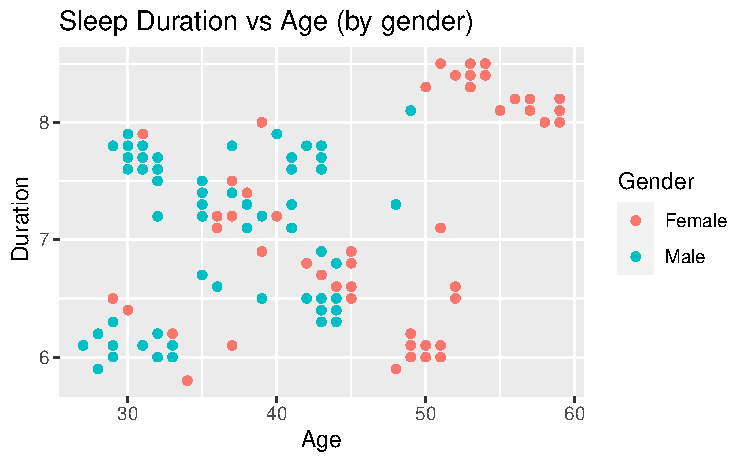
\includegraphics[width=0.7\linewidth]{SleepHelath_files/figure-latex/unnamed-chunk-5-1} \end{center}

\begin{Shaded}
\begin{Highlighting}[]
\NormalTok{model\_2 }\OtherTok{\textless{}{-}} \FunctionTok{lm}\NormalTok{(Duration }\SpecialCharTok{\textasciitilde{}}\NormalTok{ Physical,Sleep\_health\_and\_lifestyle\_dataset\_renamed)}
\end{Highlighting}
\end{Shaded}

\begin{Shaded}
\begin{Highlighting}[]
\NormalTok{model\_2}\SpecialCharTok{$}\NormalTok{coefficients}
\end{Highlighting}
\end{Shaded}

\begin{verbatim}
## (Intercept)    Physical 
## 6.652127945 0.008111349
\end{verbatim}

\begin{Shaded}
\begin{Highlighting}[]
\NormalTok{Sleep\_health\_and\_lifestyle\_dataset\_renamed }\SpecialCharTok{\%\textgreater{}\%}
  \FunctionTok{ggplot}\NormalTok{() }\SpecialCharTok{+}
  \FunctionTok{geom\_point}\NormalTok{(}\AttributeTok{mapping =} \FunctionTok{aes}\NormalTok{(}\AttributeTok{x =}\NormalTok{ Physical, }\AttributeTok{y =}\NormalTok{ Duration), }\AttributeTok{bin =} \DecValTok{10}\NormalTok{) }\SpecialCharTok{+}
  \FunctionTok{geom\_abline}\NormalTok{(}\AttributeTok{slope =}\NormalTok{ model\_2}\SpecialCharTok{$}\NormalTok{coefficients[}\DecValTok{2}\NormalTok{], }
              \AttributeTok{intercept =}\NormalTok{ model\_2}\SpecialCharTok{$}\NormalTok{coefficients[}\DecValTok{1}\NormalTok{])}\SpecialCharTok{+}
   \FunctionTok{labs}\NormalTok{(}\AttributeTok{x =} \StringTok{"Physical Activity Level"}\NormalTok{, }\AttributeTok{y =} \StringTok{"Sleep Duration"}\NormalTok{,}
                    \AttributeTok{title =} \StringTok{"scatter plot of physical activity level and sleep duration"}\NormalTok{ )}
\end{Highlighting}
\end{Shaded}

\begin{verbatim}
## Warning in geom_point(mapping = aes(x = Physical, y = Duration), bin = 10):
## Ignoring unknown parameters: `bin`
\end{verbatim}

\begin{center}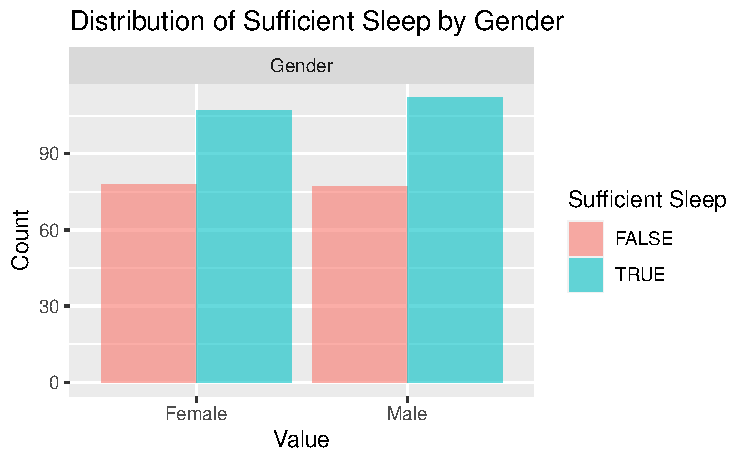
\includegraphics[width=0.7\linewidth]{SleepHelath_files/figure-latex/unnamed-chunk-8-1} \end{center}

\hypertarget{part-3}{%
\subsubsection{Part 3}\label{part-3}}

\begin{Shaded}
\begin{Highlighting}[]
\FunctionTok{library}\NormalTok{(tidyr)}
\FunctionTok{library}\NormalTok{(ggplot2)}
\FunctionTok{library}\NormalTok{(ggmosaic)}
\FunctionTok{library}\NormalTok{(dplyr)}
\NormalTok{Sleep\_health\_and\_lifestyle\_dataset }\OtherTok{\textless{}{-}} \FunctionTok{read\_csv}\NormalTok{(}\StringTok{"Sleep\_health\_and\_lifestyle\_dataset.csv"}\NormalTok{)}
\end{Highlighting}
\end{Shaded}

\begin{verbatim}
## Rows: 374 Columns: 13
## -- Column specification --------------------------------------------------------
## Delimiter: ","
## chr (5): Gender, Occupation, BMI Category, Blood Pressure, Sleep Disorder
## dbl (8): Person ID, Age, Sleep Duration, Quality of Sleep, Physical Activity...
## 
## i Use `spec()` to retrieve the full column specification for this data.
## i Specify the column types or set `show_col_types = FALSE` to quiet this message.
\end{verbatim}

\begin{Shaded}
\begin{Highlighting}[]
\NormalTok{Sleep\_health\_and\_lifestyle\_dataset\_renamed }\OtherTok{\textless{}{-}}\NormalTok{ Sleep\_health\_and\_lifestyle\_dataset }\SpecialCharTok{\%\textgreater{}\%}
  \FunctionTok{rename}\NormalTok{( }\AttributeTok{ID =} \StringTok{\textquotesingle{}Person ID\textquotesingle{}}\NormalTok{,}
          \AttributeTok{Duration =} \StringTok{\textquotesingle{}Sleep Duration\textquotesingle{}}\NormalTok{,}
          \AttributeTok{Stress =} \StringTok{\textquotesingle{}Stress Level\textquotesingle{}}\NormalTok{,}
          \AttributeTok{Physical =} \StringTok{\textquotesingle{}Physical Activity Level\textquotesingle{}}\NormalTok{ ,}
          \AttributeTok{Quality =} \StringTok{\textquotesingle{}Quality of Sleep\textquotesingle{}}\NormalTok{ ,}
          \AttributeTok{BMI=} \StringTok{\textquotesingle{}BMI Category\textquotesingle{}}\NormalTok{ ,}
          \AttributeTok{BPressure =} \StringTok{\textquotesingle{}Blood Pressure\textquotesingle{}}\NormalTok{ ,}
          \AttributeTok{HRate =} \StringTok{\textquotesingle{}Heart Rate\textquotesingle{}}\NormalTok{ ,}
          \AttributeTok{DSteps =} \StringTok{\textquotesingle{}Daily Steps\textquotesingle{}}\NormalTok{ ,}
          \AttributeTok{Disorder =} \StringTok{\textquotesingle{}Sleep Disorder\textquotesingle{}}\NormalTok{)}
\end{Highlighting}
\end{Shaded}

\begin{Shaded}
\begin{Highlighting}[]
\NormalTok{Sleep\_health\_and\_lifestyle\_dataset\_renamed}\SpecialCharTok{$}\NormalTok{BMI[Sleep\_health\_and\_lifestyle\_dataset\_renamed}\SpecialCharTok{$}\NormalTok{BMI }\SpecialCharTok{==} \StringTok{"Overweight"}\NormalTok{] }\OtherTok{\textless{}{-}} \StringTok{"Fat"}
\NormalTok{Sleep\_health\_and\_lifestyle\_dataset\_renamed}\SpecialCharTok{$}\NormalTok{BMI[Sleep\_health\_and\_lifestyle\_dataset\_renamed}\SpecialCharTok{$}\NormalTok{BMI }\SpecialCharTok{==} \StringTok{"Obese"}\NormalTok{] }\OtherTok{\textless{}{-}} \StringTok{"Fat"}
\NormalTok{Sleep\_health\_and\_lifestyle\_dataset\_renamed}\SpecialCharTok{$}\NormalTok{BMI[Sleep\_health\_and\_lifestyle\_dataset\_renamed}\SpecialCharTok{$}\NormalTok{BMI }\SpecialCharTok{==} \StringTok{"Normal Weight"}\NormalTok{] }\OtherTok{\textless{}{-}} \StringTok{"Normal"}
\end{Highlighting}
\end{Shaded}

\begin{Shaded}
\begin{Highlighting}[]
\NormalTok{Sleep\_health\_and\_lifestyle\_dataset\_renamed }\SpecialCharTok{\%\textgreater{}\%}
  \FunctionTok{select}\NormalTok{(ID, HRate, Duration, Gender, Age, Occupation, Physical, BMI, Quality) }\SpecialCharTok{\%\textgreater{}\%}
  \FunctionTok{arrange}\NormalTok{(Duration)}
\end{Highlighting}
\end{Shaded}

\begin{longtable}[]{@{}
  >{\raggedleft\arraybackslash}p{(\columnwidth - 16\tabcolsep) * \real{0.0533}}
  >{\raggedleft\arraybackslash}p{(\columnwidth - 16\tabcolsep) * \real{0.0800}}
  >{\raggedleft\arraybackslash}p{(\columnwidth - 16\tabcolsep) * \real{0.1200}}
  >{\raggedright\arraybackslash}p{(\columnwidth - 16\tabcolsep) * \real{0.0933}}
  >{\raggedleft\arraybackslash}p{(\columnwidth - 16\tabcolsep) * \real{0.0533}}
  >{\raggedright\arraybackslash}p{(\columnwidth - 16\tabcolsep) * \real{0.2800}}
  >{\raggedleft\arraybackslash}p{(\columnwidth - 16\tabcolsep) * \real{0.1200}}
  >{\raggedright\arraybackslash}p{(\columnwidth - 16\tabcolsep) * \real{0.0933}}
  >{\raggedleft\arraybackslash}p{(\columnwidth - 16\tabcolsep) * \real{0.1067}}@{}}
\toprule\noalign{}
\begin{minipage}[b]{\linewidth}\raggedleft
ID
\end{minipage} & \begin{minipage}[b]{\linewidth}\raggedleft
HRate
\end{minipage} & \begin{minipage}[b]{\linewidth}\raggedleft
Duration
\end{minipage} & \begin{minipage}[b]{\linewidth}\raggedright
Gender
\end{minipage} & \begin{minipage}[b]{\linewidth}\raggedleft
Age
\end{minipage} & \begin{minipage}[b]{\linewidth}\raggedright
Occupation
\end{minipage} & \begin{minipage}[b]{\linewidth}\raggedleft
Physical
\end{minipage} & \begin{minipage}[b]{\linewidth}\raggedright
BMI
\end{minipage} & \begin{minipage}[b]{\linewidth}\raggedleft
Quality
\end{minipage} \\
\midrule\noalign{}
\endhead
\bottomrule\noalign{}
\endlastfoot
81 & 81 & 5.8 & Female & 34 & Scientist & 32 & Fat & 4 \\
82 & 81 & 5.8 & Female & 34 & Scientist & 32 & Fat & 4 \\
4 & 85 & 5.9 & Male & 28 & Sales Representative & 30 & Fat & 4 \\
5 & 85 & 5.9 & Male & 28 & Sales Representative & 30 & Fat & 4 \\
6 & 85 & 5.9 & Male & 28 & Software Engineer & 30 & Fat & 4 \\
266 & 75 & 5.9 & Female & 48 & Nurse & 90 & Fat & 6 \\
14 & 70 & 6.0 & Male & 29 & Doctor & 30 & Normal & 6 \\
15 & 70 & 6.0 & Male & 29 & Doctor & 30 & Normal & 6 \\
16 & 70 & 6.0 & Male & 29 & Doctor & 30 & Normal & 6 \\
18 & 70 & 6.0 & Male & 29 & Doctor & 30 & Normal & 6 \\
53 & 72 & 6.0 & Male & 32 & Doctor & 30 & Normal & 6 \\
55 & 72 & 6.0 & Male & 32 & Doctor & 30 & Normal & 6 \\
56 & 72 & 6.0 & Male & 32 & Doctor & 30 & Normal & 6 \\
58 & 72 & 6.0 & Male & 32 & Doctor & 30 & Normal & 6 \\
59 & 72 & 6.0 & Male & 32 & Doctor & 30 & Normal & 6 \\
61 & 72 & 6.0 & Male & 32 & Doctor & 30 & Normal & 6 \\
62 & 72 & 6.0 & Male & 32 & Doctor & 30 & Normal & 6 \\
68 & 72 & 6.0 & Male & 33 & Doctor & 30 & Normal & 6 \\
75 & 72 & 6.0 & Male & 33 & Doctor & 30 & Normal & 6 \\
76 & 72 & 6.0 & Male & 33 & Doctor & 30 & Normal & 6 \\
77 & 72 & 6.0 & Male & 33 & Doctor & 30 & Normal & 6 \\
78 & 72 & 6.0 & Male & 33 & Doctor & 30 & Normal & 6 \\
79 & 72 & 6.0 & Male & 33 & Doctor & 30 & Normal & 6 \\
80 & 72 & 6.0 & Male & 33 & Doctor & 30 & Normal & 6 \\
269 & 75 & 6.0 & Female & 49 & Nurse & 90 & Fat & 6 \\
281 & 75 & 6.0 & Female & 50 & Nurse & 90 & Fat & 6 \\
283 & 75 & 6.0 & Female & 50 & Nurse & 90 & Fat & 6 \\
284 & 75 & 6.0 & Female & 50 & Nurse & 90 & Fat & 6 \\
285 & 75 & 6.0 & Female & 50 & Nurse & 90 & Fat & 6 \\
286 & 75 & 6.0 & Female & 50 & Nurse & 90 & Fat & 6 \\
287 & 75 & 6.0 & Female & 50 & Nurse & 90 & Fat & 6 \\
288 & 75 & 6.0 & Female & 50 & Nurse & 90 & Fat & 6 \\
289 & 75 & 6.0 & Female & 50 & Nurse & 90 & Fat & 6 \\
291 & 75 & 6.0 & Female & 50 & Nurse & 90 & Fat & 6 \\
294 & 75 & 6.0 & Female & 50 & Nurse & 90 & Fat & 6 \\
296 & 75 & 6.0 & Female & 50 & Nurse & 90 & Fat & 6 \\
304 & 75 & 6.0 & Female & 51 & Nurse & 90 & Fat & 6 \\
1 & 77 & 6.1 & Male & 27 & Software Engineer & 42 & Fat & 6 \\
11 & 70 & 6.1 & Male & 29 & Doctor & 30 & Normal & 6 \\
13 & 70 & 6.1 & Male & 29 & Doctor & 30 & Normal & 6 \\
34 & 72 & 6.1 & Male & 31 & Doctor & 30 & Normal & 6 \\
36 & 72 & 6.1 & Male & 31 & Doctor & 30 & Normal & 6 \\
37 & 72 & 6.1 & Male & 31 & Doctor & 30 & Normal & 6 \\
71 & 72 & 6.1 & Male & 33 & Doctor & 30 & Normal & 6 \\
72 & 72 & 6.1 & Male & 33 & Doctor & 30 & Normal & 6 \\
73 & 72 & 6.1 & Male & 33 & Doctor & 30 & Normal & 6 \\
74 & 72 & 6.1 & Male & 33 & Doctor & 30 & Normal & 6 \\
107 & 77 & 6.1 & Female & 37 & Nurse & 42 & Fat & 6 \\
270 & 75 & 6.1 & Female & 49 & Nurse & 90 & Fat & 6 \\
271 & 75 & 6.1 & Female & 49 & Nurse & 90 & Fat & 6 \\
272 & 75 & 6.1 & Female & 49 & Nurse & 90 & Fat & 6 \\
273 & 75 & 6.1 & Female & 49 & Nurse & 90 & Fat & 6 \\
279 & 75 & 6.1 & Female & 50 & Nurse & 90 & Fat & 6 \\
282 & 75 & 6.1 & Female & 50 & Nurse & 90 & Fat & 6 \\
290 & 75 & 6.1 & Female & 50 & Nurse & 90 & Fat & 6 \\
292 & 75 & 6.1 & Female & 50 & Nurse & 90 & Fat & 6 \\
293 & 75 & 6.1 & Female & 50 & Nurse & 90 & Fat & 6 \\
295 & 75 & 6.1 & Female & 50 & Nurse & 90 & Fat & 6 \\
297 & 75 & 6.1 & Female & 50 & Nurse & 90 & Fat & 6 \\
298 & 75 & 6.1 & Female & 50 & Nurse & 90 & Fat & 6 \\
305 & 75 & 6.1 & Female & 51 & Nurse & 90 & Fat & 6 \\
306 & 75 & 6.1 & Female & 51 & Nurse & 90 & Fat & 6 \\
2 & 75 & 6.2 & Male & 28 & Doctor & 60 & Normal & 6 \\
3 & 75 & 6.2 & Male & 28 & Doctor & 60 & Normal & 6 \\
63 & 72 & 6.2 & Male & 32 & Doctor & 30 & Normal & 6 \\
64 & 72 & 6.2 & Male & 32 & Doctor & 30 & Normal & 6 \\
65 & 72 & 6.2 & Male & 32 & Doctor & 30 & Normal & 6 \\
66 & 72 & 6.2 & Male & 32 & Doctor & 30 & Normal & 6 \\
69 & 76 & 6.2 & Female & 33 & Scientist & 50 & Fat & 6 \\
70 & 76 & 6.2 & Female & 33 & Scientist & 50 & Fat & 6 \\
268 & 75 & 6.2 & Female & 49 & Nurse & 90 & Fat & 6 \\
274 & 75 & 6.2 & Female & 49 & Nurse & 90 & Fat & 6 \\
275 & 75 & 6.2 & Female & 49 & Nurse & 90 & Fat & 6 \\
276 & 75 & 6.2 & Female & 49 & Nurse & 90 & Fat & 6 \\
7 & 82 & 6.3 & Male & 29 & Teacher & 40 & Fat & 6 \\
188 & 72 & 6.3 & Male & 43 & Salesperson & 45 & Fat & 6 \\
223 & 72 & 6.3 & Male & 44 & Salesperson & 45 & Fat & 6 \\
226 & 72 & 6.3 & Male & 44 & Salesperson & 45 & Fat & 6 \\
228 & 72 & 6.3 & Male & 44 & Salesperson & 45 & Fat & 6 \\
230 & 72 & 6.3 & Male & 44 & Salesperson & 45 & Fat & 6 \\
232 & 72 & 6.3 & Male & 44 & Salesperson & 45 & Fat & 6 \\
234 & 72 & 6.3 & Male & 44 & Salesperson & 45 & Fat & 6 \\
236 & 72 & 6.3 & Male & 44 & Salesperson & 45 & Fat & 6 \\
239 & 72 & 6.3 & Male & 44 & Salesperson & 45 & Fat & 6 \\
242 & 72 & 6.3 & Male & 44 & Salesperson & 45 & Fat & 6 \\
245 & 72 & 6.3 & Male & 44 & Salesperson & 45 & Fat & 6 \\
247 & 72 & 6.3 & Male & 44 & Salesperson & 45 & Fat & 6 \\
31 & 78 & 6.4 & Female & 30 & Nurse & 35 & Normal & 5 \\
32 & 78 & 6.4 & Female & 30 & Nurse & 35 & Normal & 5 \\
192 & 72 & 6.4 & Male & 43 & Salesperson & 45 & Fat & 6 \\
222 & 72 & 6.4 & Male & 44 & Salesperson & 45 & Fat & 6 \\
224 & 72 & 6.4 & Male & 44 & Salesperson & 45 & Fat & 6 \\
237 & 72 & 6.4 & Male & 44 & Salesperson & 45 & Fat & 6 \\
240 & 72 & 6.4 & Male & 44 & Salesperson & 45 & Fat & 6 \\
243 & 72 & 6.4 & Male & 44 & Salesperson & 45 & Fat & 6 \\
249 & 72 & 6.4 & Male & 44 & Salesperson & 45 & Fat & 6 \\
17 & 80 & 6.5 & Female & 29 & Nurse & 40 & Normal & 5 \\
19 & 80 & 6.5 & Female & 29 & Nurse & 40 & Normal & 5 \\
148 & 80 & 6.5 & Male & 39 & Engineer & 40 & Fat & 5 \\
178 & 72 & 6.5 & Male & 42 & Salesperson & 45 & Fat & 6 \\
190 & 72 & 6.5 & Male & 43 & Salesperson & 45 & Fat & 6 \\
193 & 72 & 6.5 & Male & 43 & Salesperson & 45 & Fat & 6 \\
194 & 72 & 6.5 & Male & 43 & Salesperson & 45 & Fat & 6 \\
195 & 72 & 6.5 & Male & 43 & Salesperson & 45 & Fat & 6 \\
196 & 72 & 6.5 & Male & 43 & Salesperson & 45 & Fat & 6 \\
197 & 72 & 6.5 & Male & 43 & Salesperson & 45 & Fat & 6 \\
198 & 72 & 6.5 & Male & 43 & Salesperson & 45 & Fat & 6 \\
199 & 72 & 6.5 & Male & 43 & Salesperson & 45 & Fat & 6 \\
200 & 72 & 6.5 & Male & 43 & Salesperson & 45 & Fat & 6 \\
201 & 72 & 6.5 & Male & 43 & Salesperson & 45 & Fat & 6 \\
220 & 72 & 6.5 & Male & 43 & Salesperson & 45 & Fat & 6 \\
238 & 65 & 6.5 & Female & 44 & Teacher & 45 & Fat & 7 \\
241 & 65 & 6.5 & Female & 44 & Teacher & 45 & Fat & 7 \\
244 & 65 & 6.5 & Female & 44 & Teacher & 45 & Fat & 7 \\
246 & 65 & 6.5 & Female & 44 & Teacher & 45 & Fat & 7 \\
250 & 72 & 6.5 & Male & 44 & Salesperson & 45 & Fat & 6 \\
253 & 65 & 6.5 & Female & 45 & Teacher & 45 & Fat & 7 \\
254 & 65 & 6.5 & Female & 45 & Teacher & 45 & Fat & 7 \\
255 & 65 & 6.5 & Female & 45 & Teacher & 45 & Fat & 7 \\
256 & 65 & 6.5 & Female & 45 & Teacher & 45 & Fat & 7 \\
307 & 72 & 6.5 & Female & 52 & Accountant & 45 & Fat & 7 \\
308 & 72 & 6.5 & Female & 52 & Accountant & 45 & Fat & 7 \\
104 & 74 & 6.6 & Male & 36 & Teacher & 35 & Fat & 5 \\
106 & 74 & 6.6 & Male & 36 & Teacher & 35 & Fat & 5 \\
221 & 65 & 6.6 & Female & 44 & Teacher & 45 & Fat & 7 \\
225 & 65 & 6.6 & Female & 44 & Teacher & 45 & Fat & 7 \\
227 & 65 & 6.6 & Female & 44 & Teacher & 45 & Fat & 7 \\
229 & 65 & 6.6 & Female & 44 & Teacher & 45 & Fat & 7 \\
231 & 65 & 6.6 & Female & 44 & Teacher & 45 & Fat & 7 \\
233 & 65 & 6.6 & Female & 44 & Teacher & 45 & Fat & 7 \\
235 & 65 & 6.6 & Female & 44 & Teacher & 45 & Fat & 7 \\
257 & 65 & 6.6 & Female & 45 & Teacher & 45 & Fat & 7 \\
258 & 65 & 6.6 & Female & 45 & Teacher & 45 & Fat & 7 \\
259 & 65 & 6.6 & Female & 45 & Teacher & 45 & Fat & 7 \\
260 & 65 & 6.6 & Female & 45 & Teacher & 45 & Fat & 7 \\
261 & 65 & 6.6 & Female & 45 & Teacher & 45 & Fat & 7 \\
262 & 65 & 6.6 & Female & 45 & Teacher & 45 & Fat & 7 \\
263 & 65 & 6.6 & Female & 45 & Teacher & 45 & Fat & 7 \\
309 & 72 & 6.6 & Female & 52 & Accountant & 45 & Fat & 7 \\
310 & 72 & 6.6 & Female & 52 & Accountant & 45 & Fat & 7 \\
311 & 72 & 6.6 & Female & 52 & Accountant & 45 & Fat & 7 \\
312 & 72 & 6.6 & Female & 52 & Accountant & 45 & Fat & 7 \\
83 & 70 & 6.7 & Male & 35 & Teacher & 40 & Fat & 7 \\
84 & 70 & 6.7 & Male & 35 & Teacher & 40 & Fat & 7 \\
187 & 65 & 6.7 & Female & 43 & Teacher & 45 & Fat & 7 \\
189 & 65 & 6.7 & Female & 43 & Teacher & 45 & Fat & 7 \\
191 & 65 & 6.7 & Female & 43 & Teacher & 45 & Fat & 7 \\
185 & 78 & 6.8 & Female & 42 & Teacher & 45 & Fat & 6 \\
186 & 78 & 6.8 & Female & 42 & Teacher & 45 & Fat & 6 \\
248 & 78 & 6.8 & Male & 44 & Engineer & 45 & Fat & 7 \\
251 & 65 & 6.8 & Female & 45 & Teacher & 30 & Fat & 7 \\
252 & 65 & 6.8 & Female & 45 & Teacher & 30 & Fat & 7 \\
149 & 75 & 6.9 & Female & 39 & Lawyer & 50 & Normal & 7 \\
204 & 69 & 6.9 & Male & 43 & Engineer & 47 & Normal & 6 \\
264 & 75 & 6.9 & Female & 45 & Manager & 55 & Fat & 7 \\
96 & 68 & 7.1 & Female & 36 & Accountant & 60 & Normal & 8 \\
98 & 68 & 7.1 & Female & 36 & Accountant & 60 & Normal & 8 \\
99 & 68 & 7.1 & Female & 36 & Teacher & 60 & Normal & 8 \\
100 & 68 & 7.1 & Female & 36 & Teacher & 60 & Normal & 8 \\
128 & 68 & 7.1 & Female & 38 & Accountant & 60 & Normal & 8 \\
131 & 68 & 7.1 & Female & 38 & Accountant & 60 & Normal & 8 \\
134 & 68 & 7.1 & Female & 38 & Accountant & 60 & Normal & 8 \\
137 & 68 & 7.1 & Female & 38 & Accountant & 60 & Normal & 8 \\
138 & 68 & 7.1 & Male & 38 & Lawyer & 60 & Normal & 8 \\
139 & 68 & 7.1 & Female & 38 & Accountant & 60 & Normal & 8 \\
140 & 68 & 7.1 & Male & 38 & Lawyer & 60 & Normal & 8 \\
141 & 68 & 7.1 & Female & 38 & Accountant & 60 & Normal & 8 \\
142 & 68 & 7.1 & Male & 38 & Lawyer & 60 & Normal & 8 \\
143 & 68 & 7.1 & Female & 38 & Accountant & 60 & Normal & 8 \\
144 & 68 & 7.1 & Female & 38 & Accountant & 60 & Normal & 8 \\
145 & 68 & 7.1 & Male & 38 & Lawyer & 60 & Normal & 8 \\
168 & 72 & 7.1 & Male & 41 & Lawyer & 55 & Fat & 7 \\
169 & 72 & 7.1 & Male & 41 & Lawyer & 55 & Fat & 7 \\
303 & 72 & 7.1 & Female & 51 & Nurse & 55 & Normal & 7 \\
67 & 68 & 7.2 & Male & 32 & Accountant & 50 & Normal & 8 \\
86 & 68 & 7.2 & Female & 35 & Accountant & 60 & Normal & 8 \\
87 & 65 & 7.2 & Male & 35 & Engineer & 60 & Normal & 8 \\
88 & 65 & 7.2 & Male & 35 & Engineer & 60 & Normal & 8 \\
95 & 68 & 7.2 & Female & 36 & Accountant & 60 & Normal & 8 \\
97 & 68 & 7.2 & Female & 36 & Accountant & 60 & Normal & 8 \\
101 & 68 & 7.2 & Female & 36 & Teacher & 60 & Normal & 8 \\
102 & 68 & 7.2 & Female & 36 & Teacher & 60 & Normal & 8 \\
103 & 68 & 7.2 & Female & 36 & Teacher & 60 & Normal & 8 \\
105 & 68 & 7.2 & Female & 36 & Teacher & 60 & Normal & 8 \\
111 & 68 & 7.2 & Female & 37 & Accountant & 60 & Normal & 8 \\
113 & 68 & 7.2 & Female & 37 & Accountant & 60 & Normal & 8 \\
115 & 68 & 7.2 & Female & 37 & Accountant & 60 & Normal & 8 \\
116 & 68 & 7.2 & Female & 37 & Accountant & 60 & Normal & 8 \\
117 & 68 & 7.2 & Female & 37 & Accountant & 60 & Normal & 8 \\
118 & 68 & 7.2 & Female & 37 & Accountant & 60 & Normal & 8 \\
119 & 68 & 7.2 & Female & 37 & Accountant & 60 & Normal & 8 \\
120 & 68 & 7.2 & Female & 37 & Accountant & 60 & Normal & 8 \\
121 & 68 & 7.2 & Female & 37 & Accountant & 60 & Normal & 8 \\
122 & 68 & 7.2 & Female & 37 & Accountant & 60 & Normal & 8 \\
123 & 68 & 7.2 & Female & 37 & Accountant & 60 & Normal & 8 \\
124 & 68 & 7.2 & Female & 37 & Accountant & 60 & Normal & 8 \\
125 & 68 & 7.2 & Female & 37 & Accountant & 60 & Normal & 8 \\
147 & 68 & 7.2 & Male & 39 & Lawyer & 60 & Normal & 8 \\
152 & 68 & 7.2 & Male & 39 & Lawyer & 60 & Normal & 8 \\
153 & 68 & 7.2 & Male & 39 & Lawyer & 60 & Normal & 8 \\
154 & 68 & 7.2 & Male & 39 & Lawyer & 60 & Normal & 8 \\
155 & 68 & 7.2 & Male & 39 & Lawyer & 60 & Normal & 8 \\
156 & 68 & 7.2 & Male & 39 & Lawyer & 60 & Normal & 8 \\
157 & 68 & 7.2 & Male & 39 & Lawyer & 60 & Normal & 8 \\
158 & 68 & 7.2 & Male & 39 & Lawyer & 60 & Normal & 8 \\
159 & 68 & 7.2 & Male & 39 & Lawyer & 60 & Normal & 8 \\
160 & 68 & 7.2 & Male & 39 & Lawyer & 60 & Normal & 8 \\
161 & 68 & 7.2 & Male & 39 & Lawyer & 60 & Normal & 8 \\
162 & 73 & 7.2 & Female & 40 & Accountant & 55 & Normal & 8 \\
163 & 73 & 7.2 & Female & 40 & Accountant & 55 & Normal & 8 \\
89 & 65 & 7.3 & Male & 35 & Engineer & 60 & Normal & 8 \\
90 & 65 & 7.3 & Male & 35 & Engineer & 60 & Normal & 8 \\
91 & 65 & 7.3 & Male & 35 & Engineer & 60 & Normal & 8 \\
92 & 65 & 7.3 & Male & 35 & Engineer & 60 & Normal & 8 \\
127 & 68 & 7.3 & Male & 38 & Lawyer & 60 & Normal & 8 \\
129 & 68 & 7.3 & Male & 38 & Lawyer & 60 & Normal & 8 \\
130 & 68 & 7.3 & Male & 38 & Lawyer & 60 & Normal & 8 \\
132 & 68 & 7.3 & Male & 38 & Lawyer & 60 & Normal & 8 \\
133 & 68 & 7.3 & Male & 38 & Lawyer & 60 & Normal & 8 \\
135 & 68 & 7.3 & Male & 38 & Lawyer & 60 & Normal & 8 \\
136 & 68 & 7.3 & Male & 38 & Lawyer & 60 & Normal & 8 \\
167 & 72 & 7.3 & Male & 41 & Engineer & 70 & Normal & 8 \\
265 & 83 & 7.3 & Male & 48 & Doctor & 65 & Fat & 7 \\
267 & 83 & 7.3 & Male & 48 & Doctor & 65 & Fat & 7 \\
94 & 84 & 7.4 & Male & 35 & Lawyer & 60 & Fat & 7 \\
110 & 68 & 7.4 & Male & 37 & Lawyer & 60 & Normal & 8 \\
112 & 68 & 7.4 & Male & 37 & Lawyer & 60 & Normal & 8 \\
114 & 68 & 7.4 & Male & 37 & Lawyer & 60 & Normal & 8 \\
146 & 84 & 7.4 & Female & 38 & Lawyer & 60 & Fat & 7 \\
51 & 70 & 7.5 & Male & 32 & Engineer & 45 & Normal & 8 \\
52 & 70 & 7.5 & Male & 32 & Engineer & 45 & Normal & 8 \\
85 & 70 & 7.5 & Male & 35 & Software Engineer & 60 & Normal & 8 \\
93 & 70 & 7.5 & Male & 35 & Software Engineer & 60 & Normal & 8 \\
126 & 70 & 7.5 & Female & 37 & Nurse & 60 & Normal & 8 \\
20 & 70 & 7.6 & Male & 30 & Doctor & 75 & Normal & 7 \\
38 & 70 & 7.6 & Male & 31 & Doctor & 75 & Normal & 7 \\
39 & 70 & 7.6 & Male & 31 & Doctor & 75 & Normal & 7 \\
40 & 70 & 7.6 & Male & 31 & Doctor & 75 & Normal & 7 \\
54 & 70 & 7.6 & Male & 32 & Doctor & 75 & Normal & 7 \\
166 & 70 & 7.6 & Male & 41 & Lawyer & 90 & Normal & 8 \\
175 & 70 & 7.6 & Male & 41 & Lawyer & 90 & Normal & 8 \\
176 & 70 & 7.6 & Male & 41 & Lawyer & 90 & Normal & 8 \\
177 & 70 & 7.6 & Male & 41 & Lawyer & 90 & Normal & 8 \\
205 & 68 & 7.6 & Male & 43 & Engineer & 75 & Fat & 8 \\
21 & 70 & 7.7 & Male & 30 & Doctor & 75 & Normal & 7 \\
22 & 70 & 7.7 & Male & 30 & Doctor & 75 & Normal & 7 \\
23 & 70 & 7.7 & Male & 30 & Doctor & 75 & Normal & 7 \\
24 & 70 & 7.7 & Male & 30 & Doctor & 75 & Normal & 7 \\
35 & 70 & 7.7 & Male & 31 & Doctor & 75 & Normal & 7 \\
41 & 70 & 7.7 & Male & 31 & Doctor & 75 & Normal & 7 \\
42 & 70 & 7.7 & Male & 31 & Doctor & 75 & Normal & 7 \\
43 & 70 & 7.7 & Male & 31 & Doctor & 75 & Normal & 7 \\
45 & 70 & 7.7 & Male & 31 & Doctor & 75 & Normal & 7 \\
47 & 70 & 7.7 & Male & 31 & Doctor & 75 & Normal & 7 \\
49 & 70 & 7.7 & Male & 31 & Doctor & 75 & Normal & 7 \\
50 & 70 & 7.7 & Male & 31 & Doctor & 75 & Normal & 7 \\
57 & 70 & 7.7 & Male & 32 & Doctor & 75 & Normal & 7 \\
60 & 70 & 7.7 & Male & 32 & Doctor & 75 & Normal & 7 \\
170 & 70 & 7.7 & Male & 41 & Lawyer & 90 & Normal & 8 \\
171 & 70 & 7.7 & Male & 41 & Lawyer & 90 & Normal & 8 \\
172 & 70 & 7.7 & Male & 41 & Lawyer & 90 & Normal & 8 \\
173 & 70 & 7.7 & Male & 41 & Lawyer & 90 & Normal & 8 \\
174 & 70 & 7.7 & Male & 41 & Lawyer & 90 & Normal & 8 \\
206 & 70 & 7.7 & Male & 43 & Engineer & 90 & Normal & 8 \\
207 & 70 & 7.7 & Male & 43 & Engineer & 90 & Normal & 8 \\
208 & 70 & 7.7 & Male & 43 & Engineer & 90 & Normal & 8 \\
209 & 70 & 7.7 & Male & 43 & Engineer & 90 & Normal & 8 \\
211 & 70 & 7.7 & Male & 43 & Engineer & 90 & Normal & 8 \\
8 & 70 & 7.8 & Male & 29 & Doctor & 75 & Normal & 7 \\
9 & 70 & 7.8 & Male & 29 & Doctor & 75 & Normal & 7 \\
10 & 70 & 7.8 & Male & 29 & Doctor & 75 & Normal & 7 \\
12 & 70 & 7.8 & Male & 29 & Doctor & 75 & Normal & 7 \\
25 & 70 & 7.8 & Male & 30 & Doctor & 75 & Normal & 7 \\
27 & 70 & 7.8 & Male & 30 & Doctor & 75 & Normal & 7 \\
44 & 70 & 7.8 & Male & 31 & Doctor & 75 & Normal & 7 \\
46 & 70 & 7.8 & Male & 31 & Doctor & 75 & Normal & 7 \\
48 & 70 & 7.8 & Male & 31 & Doctor & 75 & Normal & 7 \\
108 & 68 & 7.8 & Male & 37 & Engineer & 70 & Normal & 8 \\
109 & 68 & 7.8 & Male & 37 & Engineer & 70 & Normal & 8 \\
179 & 70 & 7.8 & Male & 42 & Lawyer & 90 & Normal & 8 \\
180 & 70 & 7.8 & Male & 42 & Lawyer & 90 & Normal & 8 \\
181 & 70 & 7.8 & Male & 42 & Lawyer & 90 & Normal & 8 \\
182 & 70 & 7.8 & Male & 42 & Lawyer & 90 & Normal & 8 \\
183 & 70 & 7.8 & Male & 42 & Lawyer & 90 & Normal & 8 \\
184 & 70 & 7.8 & Male & 42 & Lawyer & 90 & Normal & 8 \\
202 & 70 & 7.8 & Male & 43 & Engineer & 90 & Normal & 8 \\
203 & 70 & 7.8 & Male & 43 & Engineer & 90 & Normal & 8 \\
210 & 70 & 7.8 & Male & 43 & Engineer & 90 & Normal & 8 \\
212 & 70 & 7.8 & Male & 43 & Engineer & 90 & Normal & 8 \\
213 & 70 & 7.8 & Male & 43 & Engineer & 90 & Normal & 8 \\
214 & 70 & 7.8 & Male & 43 & Engineer & 90 & Normal & 8 \\
215 & 70 & 7.8 & Male & 43 & Engineer & 90 & Normal & 8 \\
216 & 70 & 7.8 & Male & 43 & Engineer & 90 & Normal & 8 \\
217 & 70 & 7.8 & Male & 43 & Engineer & 90 & Normal & 8 \\
218 & 70 & 7.8 & Male & 43 & Engineer & 90 & Normal & 8 \\
219 & 70 & 7.8 & Male & 43 & Engineer & 90 & Normal & 8 \\
26 & 70 & 7.9 & Male & 30 & Doctor & 75 & Normal & 7 \\
28 & 70 & 7.9 & Male & 30 & Doctor & 75 & Normal & 7 \\
29 & 70 & 7.9 & Male & 30 & Doctor & 75 & Normal & 7 \\
30 & 70 & 7.9 & Male & 30 & Doctor & 75 & Normal & 7 \\
33 & 69 & 7.9 & Female & 31 & Nurse & 75 & Normal & 8 \\
164 & 68 & 7.9 & Male & 40 & Lawyer & 90 & Normal & 8 \\
165 & 68 & 7.9 & Male & 40 & Lawyer & 90 & Normal & 8 \\
150 & 67 & 8.0 & Female & 39 & Accountant & 80 & Normal & 9 \\
151 & 67 & 8.0 & Female & 39 & Accountant & 80 & Normal & 9 \\
353 & 68 & 8.0 & Female & 58 & Nurse & 75 & Fat & 9 \\
354 & 68 & 8.0 & Female & 58 & Nurse & 75 & Fat & 9 \\
355 & 68 & 8.0 & Female & 58 & Nurse & 75 & Fat & 9 \\
356 & 68 & 8.0 & Female & 58 & Nurse & 75 & Fat & 9 \\
357 & 68 & 8.0 & Female & 58 & Nurse & 75 & Fat & 9 \\
358 & 68 & 8.0 & Female & 58 & Nurse & 75 & Fat & 9 \\
359 & 68 & 8.0 & Female & 59 & Nurse & 75 & Fat & 9 \\
365 & 68 & 8.0 & Female & 59 & Nurse & 75 & Fat & 9 \\
366 & 68 & 8.0 & Female & 59 & Nurse & 75 & Fat & 9 \\
368 & 68 & 8.0 & Female & 59 & Nurse & 75 & Fat & 9 \\
371 & 68 & 8.0 & Female & 59 & Nurse & 75 & Fat & 9 \\
277 & 86 & 8.1 & Male & 49 & Doctor & 85 & Fat & 9 \\
278 & 86 & 8.1 & Male & 49 & Doctor & 85 & Fat & 9 \\
340 & 72 & 8.1 & Female & 55 & Nurse & 75 & Fat & 9 \\
341 & 72 & 8.1 & Female & 55 & Nurse & 75 & Fat & 9 \\
344 & 68 & 8.1 & Female & 57 & Nurse & 75 & Fat & 9 \\
350 & 68 & 8.1 & Female & 57 & Nurse & 75 & Fat & 9 \\
351 & 68 & 8.1 & Female & 57 & Nurse & 75 & Fat & 9 \\
352 & 68 & 8.1 & Female & 57 & Nurse & 75 & Fat & 9 \\
360 & 68 & 8.1 & Female & 59 & Nurse & 75 & Fat & 9 \\
367 & 68 & 8.1 & Female & 59 & Nurse & 75 & Fat & 9 \\
369 & 68 & 8.1 & Female & 59 & Nurse & 75 & Fat & 9 \\
370 & 68 & 8.1 & Female & 59 & Nurse & 75 & Fat & 9 \\
372 & 68 & 8.1 & Female & 59 & Nurse & 75 & Fat & 9 \\
373 & 68 & 8.1 & Female & 59 & Nurse & 75 & Fat & 9 \\
374 & 68 & 8.1 & Female & 59 & Nurse & 75 & Fat & 9 \\
342 & 65 & 8.2 & Female & 56 & Doctor & 90 & Normal & 9 \\
343 & 65 & 8.2 & Female & 56 & Doctor & 90 & Normal & 9 \\
345 & 68 & 8.2 & Female & 57 & Nurse & 75 & Fat & 9 \\
346 & 68 & 8.2 & Female & 57 & Nurse & 75 & Fat & 9 \\
347 & 68 & 8.2 & Female & 57 & Nurse & 75 & Fat & 9 \\
348 & 68 & 8.2 & Female & 57 & Nurse & 75 & Fat & 9 \\
349 & 68 & 8.2 & Female & 57 & Nurse & 75 & Fat & 9 \\
361 & 68 & 8.2 & Female & 59 & Nurse & 75 & Fat & 9 \\
362 & 68 & 8.2 & Female & 59 & Nurse & 75 & Fat & 9 \\
363 & 68 & 8.2 & Female & 59 & Nurse & 75 & Fat & 9 \\
364 & 68 & 8.2 & Female & 59 & Nurse & 75 & Fat & 9 \\
280 & 65 & 8.3 & Female & 50 & Engineer & 30 & Normal & 9 \\
316 & 65 & 8.3 & Female & 53 & Engineer & 30 & Normal & 9 \\
325 & 65 & 8.3 & Female & 53 & Engineer & 30 & Normal & 9 \\
327 & 65 & 8.3 & Female & 53 & Engineer & 30 & Normal & 9 \\
329 & 65 & 8.3 & Female & 53 & Engineer & 30 & Normal & 9 \\
313 & 65 & 8.4 & Female & 52 & Engineer & 30 & Normal & 9 \\
314 & 65 & 8.4 & Female & 52 & Engineer & 30 & Normal & 9 \\
315 & 65 & 8.4 & Female & 52 & Engineer & 30 & Normal & 9 \\
319 & 65 & 8.4 & Female & 53 & Engineer & 30 & Normal & 9 \\
320 & 65 & 8.4 & Female & 53 & Engineer & 30 & Normal & 9 \\
322 & 65 & 8.4 & Female & 53 & Engineer & 30 & Normal & 9 \\
323 & 65 & 8.4 & Female & 53 & Engineer & 30 & Normal & 9 \\
332 & 65 & 8.4 & Female & 53 & Engineer & 30 & Normal & 9 \\
333 & 65 & 8.4 & Female & 54 & Engineer & 30 & Normal & 9 \\
334 & 65 & 8.4 & Female & 54 & Engineer & 30 & Normal & 9 \\
335 & 65 & 8.4 & Female & 54 & Engineer & 30 & Normal & 9 \\
336 & 65 & 8.4 & Female & 54 & Engineer & 30 & Normal & 9 \\
337 & 65 & 8.4 & Female & 54 & Engineer & 30 & Normal & 9 \\
338 & 65 & 8.4 & Female & 54 & Engineer & 30 & Normal & 9 \\
299 & 65 & 8.5 & Female & 51 & Engineer & 30 & Normal & 9 \\
300 & 65 & 8.5 & Female & 51 & Engineer & 30 & Normal & 9 \\
301 & 65 & 8.5 & Female & 51 & Engineer & 30 & Normal & 9 \\
302 & 65 & 8.5 & Female & 51 & Engineer & 30 & Normal & 9 \\
317 & 65 & 8.5 & Female & 53 & Engineer & 30 & Normal & 9 \\
318 & 65 & 8.5 & Female & 53 & Engineer & 30 & Normal & 9 \\
321 & 65 & 8.5 & Female & 53 & Engineer & 30 & Normal & 9 \\
324 & 65 & 8.5 & Female & 53 & Engineer & 30 & Normal & 9 \\
326 & 65 & 8.5 & Female & 53 & Engineer & 30 & Normal & 9 \\
328 & 65 & 8.5 & Female & 53 & Engineer & 30 & Normal & 9 \\
330 & 65 & 8.5 & Female & 53 & Engineer & 30 & Normal & 9 \\
331 & 65 & 8.5 & Female & 53 & Engineer & 30 & Normal & 9 \\
339 & 65 & 8.5 & Female & 54 & Engineer & 30 & Normal & 9 \\
\end{longtable}

\begin{Shaded}
\begin{Highlighting}[]
\NormalTok{Sleep\_health\_and\_lifestyle\_dataset\_renamed }\SpecialCharTok{\%\textgreater{}\%}
 \FunctionTok{select}\NormalTok{(ID, HRate, Duration, Gender, Age, Occupation, Physical, BMI, Quality) }\SpecialCharTok{\%\textgreater{}\%}
  \FunctionTok{arrange}\NormalTok{(Duration) }\SpecialCharTok{\%\textgreater{}\%}
  \FunctionTok{filter}\NormalTok{(Gender }\SpecialCharTok{==} \StringTok{\textquotesingle{}Female\textquotesingle{}}\NormalTok{)}
\end{Highlighting}
\end{Shaded}

\begin{longtable}[]{@{}
  >{\raggedleft\arraybackslash}p{(\columnwidth - 16\tabcolsep) * \real{0.0615}}
  >{\raggedleft\arraybackslash}p{(\columnwidth - 16\tabcolsep) * \real{0.0923}}
  >{\raggedleft\arraybackslash}p{(\columnwidth - 16\tabcolsep) * \real{0.1385}}
  >{\raggedright\arraybackslash}p{(\columnwidth - 16\tabcolsep) * \real{0.1077}}
  >{\raggedleft\arraybackslash}p{(\columnwidth - 16\tabcolsep) * \real{0.0615}}
  >{\raggedright\arraybackslash}p{(\columnwidth - 16\tabcolsep) * \real{0.1692}}
  >{\raggedleft\arraybackslash}p{(\columnwidth - 16\tabcolsep) * \real{0.1385}}
  >{\raggedright\arraybackslash}p{(\columnwidth - 16\tabcolsep) * \real{0.1077}}
  >{\raggedleft\arraybackslash}p{(\columnwidth - 16\tabcolsep) * \real{0.1231}}@{}}
\toprule\noalign{}
\begin{minipage}[b]{\linewidth}\raggedleft
ID
\end{minipage} & \begin{minipage}[b]{\linewidth}\raggedleft
HRate
\end{minipage} & \begin{minipage}[b]{\linewidth}\raggedleft
Duration
\end{minipage} & \begin{minipage}[b]{\linewidth}\raggedright
Gender
\end{minipage} & \begin{minipage}[b]{\linewidth}\raggedleft
Age
\end{minipage} & \begin{minipage}[b]{\linewidth}\raggedright
Occupation
\end{minipage} & \begin{minipage}[b]{\linewidth}\raggedleft
Physical
\end{minipage} & \begin{minipage}[b]{\linewidth}\raggedright
BMI
\end{minipage} & \begin{minipage}[b]{\linewidth}\raggedleft
Quality
\end{minipage} \\
\midrule\noalign{}
\endhead
\bottomrule\noalign{}
\endlastfoot
81 & 81 & 5.8 & Female & 34 & Scientist & 32 & Fat & 4 \\
82 & 81 & 5.8 & Female & 34 & Scientist & 32 & Fat & 4 \\
266 & 75 & 5.9 & Female & 48 & Nurse & 90 & Fat & 6 \\
269 & 75 & 6.0 & Female & 49 & Nurse & 90 & Fat & 6 \\
281 & 75 & 6.0 & Female & 50 & Nurse & 90 & Fat & 6 \\
283 & 75 & 6.0 & Female & 50 & Nurse & 90 & Fat & 6 \\
284 & 75 & 6.0 & Female & 50 & Nurse & 90 & Fat & 6 \\
285 & 75 & 6.0 & Female & 50 & Nurse & 90 & Fat & 6 \\
286 & 75 & 6.0 & Female & 50 & Nurse & 90 & Fat & 6 \\
287 & 75 & 6.0 & Female & 50 & Nurse & 90 & Fat & 6 \\
288 & 75 & 6.0 & Female & 50 & Nurse & 90 & Fat & 6 \\
289 & 75 & 6.0 & Female & 50 & Nurse & 90 & Fat & 6 \\
291 & 75 & 6.0 & Female & 50 & Nurse & 90 & Fat & 6 \\
294 & 75 & 6.0 & Female & 50 & Nurse & 90 & Fat & 6 \\
296 & 75 & 6.0 & Female & 50 & Nurse & 90 & Fat & 6 \\
304 & 75 & 6.0 & Female & 51 & Nurse & 90 & Fat & 6 \\
107 & 77 & 6.1 & Female & 37 & Nurse & 42 & Fat & 6 \\
270 & 75 & 6.1 & Female & 49 & Nurse & 90 & Fat & 6 \\
271 & 75 & 6.1 & Female & 49 & Nurse & 90 & Fat & 6 \\
272 & 75 & 6.1 & Female & 49 & Nurse & 90 & Fat & 6 \\
273 & 75 & 6.1 & Female & 49 & Nurse & 90 & Fat & 6 \\
279 & 75 & 6.1 & Female & 50 & Nurse & 90 & Fat & 6 \\
282 & 75 & 6.1 & Female & 50 & Nurse & 90 & Fat & 6 \\
290 & 75 & 6.1 & Female & 50 & Nurse & 90 & Fat & 6 \\
292 & 75 & 6.1 & Female & 50 & Nurse & 90 & Fat & 6 \\
293 & 75 & 6.1 & Female & 50 & Nurse & 90 & Fat & 6 \\
295 & 75 & 6.1 & Female & 50 & Nurse & 90 & Fat & 6 \\
297 & 75 & 6.1 & Female & 50 & Nurse & 90 & Fat & 6 \\
298 & 75 & 6.1 & Female & 50 & Nurse & 90 & Fat & 6 \\
305 & 75 & 6.1 & Female & 51 & Nurse & 90 & Fat & 6 \\
306 & 75 & 6.1 & Female & 51 & Nurse & 90 & Fat & 6 \\
69 & 76 & 6.2 & Female & 33 & Scientist & 50 & Fat & 6 \\
70 & 76 & 6.2 & Female & 33 & Scientist & 50 & Fat & 6 \\
268 & 75 & 6.2 & Female & 49 & Nurse & 90 & Fat & 6 \\
274 & 75 & 6.2 & Female & 49 & Nurse & 90 & Fat & 6 \\
275 & 75 & 6.2 & Female & 49 & Nurse & 90 & Fat & 6 \\
276 & 75 & 6.2 & Female & 49 & Nurse & 90 & Fat & 6 \\
31 & 78 & 6.4 & Female & 30 & Nurse & 35 & Normal & 5 \\
32 & 78 & 6.4 & Female & 30 & Nurse & 35 & Normal & 5 \\
17 & 80 & 6.5 & Female & 29 & Nurse & 40 & Normal & 5 \\
19 & 80 & 6.5 & Female & 29 & Nurse & 40 & Normal & 5 \\
238 & 65 & 6.5 & Female & 44 & Teacher & 45 & Fat & 7 \\
241 & 65 & 6.5 & Female & 44 & Teacher & 45 & Fat & 7 \\
244 & 65 & 6.5 & Female & 44 & Teacher & 45 & Fat & 7 \\
246 & 65 & 6.5 & Female & 44 & Teacher & 45 & Fat & 7 \\
253 & 65 & 6.5 & Female & 45 & Teacher & 45 & Fat & 7 \\
254 & 65 & 6.5 & Female & 45 & Teacher & 45 & Fat & 7 \\
255 & 65 & 6.5 & Female & 45 & Teacher & 45 & Fat & 7 \\
256 & 65 & 6.5 & Female & 45 & Teacher & 45 & Fat & 7 \\
307 & 72 & 6.5 & Female & 52 & Accountant & 45 & Fat & 7 \\
308 & 72 & 6.5 & Female & 52 & Accountant & 45 & Fat & 7 \\
221 & 65 & 6.6 & Female & 44 & Teacher & 45 & Fat & 7 \\
225 & 65 & 6.6 & Female & 44 & Teacher & 45 & Fat & 7 \\
227 & 65 & 6.6 & Female & 44 & Teacher & 45 & Fat & 7 \\
229 & 65 & 6.6 & Female & 44 & Teacher & 45 & Fat & 7 \\
231 & 65 & 6.6 & Female & 44 & Teacher & 45 & Fat & 7 \\
233 & 65 & 6.6 & Female & 44 & Teacher & 45 & Fat & 7 \\
235 & 65 & 6.6 & Female & 44 & Teacher & 45 & Fat & 7 \\
257 & 65 & 6.6 & Female & 45 & Teacher & 45 & Fat & 7 \\
258 & 65 & 6.6 & Female & 45 & Teacher & 45 & Fat & 7 \\
259 & 65 & 6.6 & Female & 45 & Teacher & 45 & Fat & 7 \\
260 & 65 & 6.6 & Female & 45 & Teacher & 45 & Fat & 7 \\
261 & 65 & 6.6 & Female & 45 & Teacher & 45 & Fat & 7 \\
262 & 65 & 6.6 & Female & 45 & Teacher & 45 & Fat & 7 \\
263 & 65 & 6.6 & Female & 45 & Teacher & 45 & Fat & 7 \\
309 & 72 & 6.6 & Female & 52 & Accountant & 45 & Fat & 7 \\
310 & 72 & 6.6 & Female & 52 & Accountant & 45 & Fat & 7 \\
311 & 72 & 6.6 & Female & 52 & Accountant & 45 & Fat & 7 \\
312 & 72 & 6.6 & Female & 52 & Accountant & 45 & Fat & 7 \\
187 & 65 & 6.7 & Female & 43 & Teacher & 45 & Fat & 7 \\
189 & 65 & 6.7 & Female & 43 & Teacher & 45 & Fat & 7 \\
191 & 65 & 6.7 & Female & 43 & Teacher & 45 & Fat & 7 \\
185 & 78 & 6.8 & Female & 42 & Teacher & 45 & Fat & 6 \\
186 & 78 & 6.8 & Female & 42 & Teacher & 45 & Fat & 6 \\
251 & 65 & 6.8 & Female & 45 & Teacher & 30 & Fat & 7 \\
252 & 65 & 6.8 & Female & 45 & Teacher & 30 & Fat & 7 \\
149 & 75 & 6.9 & Female & 39 & Lawyer & 50 & Normal & 7 \\
264 & 75 & 6.9 & Female & 45 & Manager & 55 & Fat & 7 \\
96 & 68 & 7.1 & Female & 36 & Accountant & 60 & Normal & 8 \\
98 & 68 & 7.1 & Female & 36 & Accountant & 60 & Normal & 8 \\
99 & 68 & 7.1 & Female & 36 & Teacher & 60 & Normal & 8 \\
100 & 68 & 7.1 & Female & 36 & Teacher & 60 & Normal & 8 \\
128 & 68 & 7.1 & Female & 38 & Accountant & 60 & Normal & 8 \\
131 & 68 & 7.1 & Female & 38 & Accountant & 60 & Normal & 8 \\
134 & 68 & 7.1 & Female & 38 & Accountant & 60 & Normal & 8 \\
137 & 68 & 7.1 & Female & 38 & Accountant & 60 & Normal & 8 \\
139 & 68 & 7.1 & Female & 38 & Accountant & 60 & Normal & 8 \\
141 & 68 & 7.1 & Female & 38 & Accountant & 60 & Normal & 8 \\
143 & 68 & 7.1 & Female & 38 & Accountant & 60 & Normal & 8 \\
144 & 68 & 7.1 & Female & 38 & Accountant & 60 & Normal & 8 \\
303 & 72 & 7.1 & Female & 51 & Nurse & 55 & Normal & 7 \\
86 & 68 & 7.2 & Female & 35 & Accountant & 60 & Normal & 8 \\
95 & 68 & 7.2 & Female & 36 & Accountant & 60 & Normal & 8 \\
97 & 68 & 7.2 & Female & 36 & Accountant & 60 & Normal & 8 \\
101 & 68 & 7.2 & Female & 36 & Teacher & 60 & Normal & 8 \\
102 & 68 & 7.2 & Female & 36 & Teacher & 60 & Normal & 8 \\
103 & 68 & 7.2 & Female & 36 & Teacher & 60 & Normal & 8 \\
105 & 68 & 7.2 & Female & 36 & Teacher & 60 & Normal & 8 \\
111 & 68 & 7.2 & Female & 37 & Accountant & 60 & Normal & 8 \\
113 & 68 & 7.2 & Female & 37 & Accountant & 60 & Normal & 8 \\
115 & 68 & 7.2 & Female & 37 & Accountant & 60 & Normal & 8 \\
116 & 68 & 7.2 & Female & 37 & Accountant & 60 & Normal & 8 \\
117 & 68 & 7.2 & Female & 37 & Accountant & 60 & Normal & 8 \\
118 & 68 & 7.2 & Female & 37 & Accountant & 60 & Normal & 8 \\
119 & 68 & 7.2 & Female & 37 & Accountant & 60 & Normal & 8 \\
120 & 68 & 7.2 & Female & 37 & Accountant & 60 & Normal & 8 \\
121 & 68 & 7.2 & Female & 37 & Accountant & 60 & Normal & 8 \\
122 & 68 & 7.2 & Female & 37 & Accountant & 60 & Normal & 8 \\
123 & 68 & 7.2 & Female & 37 & Accountant & 60 & Normal & 8 \\
124 & 68 & 7.2 & Female & 37 & Accountant & 60 & Normal & 8 \\
125 & 68 & 7.2 & Female & 37 & Accountant & 60 & Normal & 8 \\
162 & 73 & 7.2 & Female & 40 & Accountant & 55 & Normal & 8 \\
163 & 73 & 7.2 & Female & 40 & Accountant & 55 & Normal & 8 \\
146 & 84 & 7.4 & Female & 38 & Lawyer & 60 & Fat & 7 \\
126 & 70 & 7.5 & Female & 37 & Nurse & 60 & Normal & 8 \\
33 & 69 & 7.9 & Female & 31 & Nurse & 75 & Normal & 8 \\
150 & 67 & 8.0 & Female & 39 & Accountant & 80 & Normal & 9 \\
151 & 67 & 8.0 & Female & 39 & Accountant & 80 & Normal & 9 \\
353 & 68 & 8.0 & Female & 58 & Nurse & 75 & Fat & 9 \\
354 & 68 & 8.0 & Female & 58 & Nurse & 75 & Fat & 9 \\
355 & 68 & 8.0 & Female & 58 & Nurse & 75 & Fat & 9 \\
356 & 68 & 8.0 & Female & 58 & Nurse & 75 & Fat & 9 \\
357 & 68 & 8.0 & Female & 58 & Nurse & 75 & Fat & 9 \\
358 & 68 & 8.0 & Female & 58 & Nurse & 75 & Fat & 9 \\
359 & 68 & 8.0 & Female & 59 & Nurse & 75 & Fat & 9 \\
365 & 68 & 8.0 & Female & 59 & Nurse & 75 & Fat & 9 \\
366 & 68 & 8.0 & Female & 59 & Nurse & 75 & Fat & 9 \\
368 & 68 & 8.0 & Female & 59 & Nurse & 75 & Fat & 9 \\
371 & 68 & 8.0 & Female & 59 & Nurse & 75 & Fat & 9 \\
340 & 72 & 8.1 & Female & 55 & Nurse & 75 & Fat & 9 \\
341 & 72 & 8.1 & Female & 55 & Nurse & 75 & Fat & 9 \\
344 & 68 & 8.1 & Female & 57 & Nurse & 75 & Fat & 9 \\
350 & 68 & 8.1 & Female & 57 & Nurse & 75 & Fat & 9 \\
351 & 68 & 8.1 & Female & 57 & Nurse & 75 & Fat & 9 \\
352 & 68 & 8.1 & Female & 57 & Nurse & 75 & Fat & 9 \\
360 & 68 & 8.1 & Female & 59 & Nurse & 75 & Fat & 9 \\
367 & 68 & 8.1 & Female & 59 & Nurse & 75 & Fat & 9 \\
369 & 68 & 8.1 & Female & 59 & Nurse & 75 & Fat & 9 \\
370 & 68 & 8.1 & Female & 59 & Nurse & 75 & Fat & 9 \\
372 & 68 & 8.1 & Female & 59 & Nurse & 75 & Fat & 9 \\
373 & 68 & 8.1 & Female & 59 & Nurse & 75 & Fat & 9 \\
374 & 68 & 8.1 & Female & 59 & Nurse & 75 & Fat & 9 \\
342 & 65 & 8.2 & Female & 56 & Doctor & 90 & Normal & 9 \\
343 & 65 & 8.2 & Female & 56 & Doctor & 90 & Normal & 9 \\
345 & 68 & 8.2 & Female & 57 & Nurse & 75 & Fat & 9 \\
346 & 68 & 8.2 & Female & 57 & Nurse & 75 & Fat & 9 \\
347 & 68 & 8.2 & Female & 57 & Nurse & 75 & Fat & 9 \\
348 & 68 & 8.2 & Female & 57 & Nurse & 75 & Fat & 9 \\
349 & 68 & 8.2 & Female & 57 & Nurse & 75 & Fat & 9 \\
361 & 68 & 8.2 & Female & 59 & Nurse & 75 & Fat & 9 \\
362 & 68 & 8.2 & Female & 59 & Nurse & 75 & Fat & 9 \\
363 & 68 & 8.2 & Female & 59 & Nurse & 75 & Fat & 9 \\
364 & 68 & 8.2 & Female & 59 & Nurse & 75 & Fat & 9 \\
280 & 65 & 8.3 & Female & 50 & Engineer & 30 & Normal & 9 \\
316 & 65 & 8.3 & Female & 53 & Engineer & 30 & Normal & 9 \\
325 & 65 & 8.3 & Female & 53 & Engineer & 30 & Normal & 9 \\
327 & 65 & 8.3 & Female & 53 & Engineer & 30 & Normal & 9 \\
329 & 65 & 8.3 & Female & 53 & Engineer & 30 & Normal & 9 \\
313 & 65 & 8.4 & Female & 52 & Engineer & 30 & Normal & 9 \\
314 & 65 & 8.4 & Female & 52 & Engineer & 30 & Normal & 9 \\
315 & 65 & 8.4 & Female & 52 & Engineer & 30 & Normal & 9 \\
319 & 65 & 8.4 & Female & 53 & Engineer & 30 & Normal & 9 \\
320 & 65 & 8.4 & Female & 53 & Engineer & 30 & Normal & 9 \\
322 & 65 & 8.4 & Female & 53 & Engineer & 30 & Normal & 9 \\
323 & 65 & 8.4 & Female & 53 & Engineer & 30 & Normal & 9 \\
332 & 65 & 8.4 & Female & 53 & Engineer & 30 & Normal & 9 \\
333 & 65 & 8.4 & Female & 54 & Engineer & 30 & Normal & 9 \\
334 & 65 & 8.4 & Female & 54 & Engineer & 30 & Normal & 9 \\
335 & 65 & 8.4 & Female & 54 & Engineer & 30 & Normal & 9 \\
336 & 65 & 8.4 & Female & 54 & Engineer & 30 & Normal & 9 \\
337 & 65 & 8.4 & Female & 54 & Engineer & 30 & Normal & 9 \\
338 & 65 & 8.4 & Female & 54 & Engineer & 30 & Normal & 9 \\
299 & 65 & 8.5 & Female & 51 & Engineer & 30 & Normal & 9 \\
300 & 65 & 8.5 & Female & 51 & Engineer & 30 & Normal & 9 \\
301 & 65 & 8.5 & Female & 51 & Engineer & 30 & Normal & 9 \\
302 & 65 & 8.5 & Female & 51 & Engineer & 30 & Normal & 9 \\
317 & 65 & 8.5 & Female & 53 & Engineer & 30 & Normal & 9 \\
318 & 65 & 8.5 & Female & 53 & Engineer & 30 & Normal & 9 \\
321 & 65 & 8.5 & Female & 53 & Engineer & 30 & Normal & 9 \\
324 & 65 & 8.5 & Female & 53 & Engineer & 30 & Normal & 9 \\
326 & 65 & 8.5 & Female & 53 & Engineer & 30 & Normal & 9 \\
328 & 65 & 8.5 & Female & 53 & Engineer & 30 & Normal & 9 \\
330 & 65 & 8.5 & Female & 53 & Engineer & 30 & Normal & 9 \\
331 & 65 & 8.5 & Female & 53 & Engineer & 30 & Normal & 9 \\
339 & 65 & 8.5 & Female & 54 & Engineer & 30 & Normal & 9 \\
\end{longtable}

\begin{Shaded}
\begin{Highlighting}[]
\NormalTok{Sleep\_health\_and\_lifestyle\_dataset\_renamed }\SpecialCharTok{\%\textgreater{}\%}
 \FunctionTok{select}\NormalTok{(ID, HRate, Duration, Gender, Age, Occupation, Physical, BMI, Quality) }\SpecialCharTok{\%\textgreater{}\%}
  \FunctionTok{arrange}\NormalTok{(Duration) }\SpecialCharTok{\%\textgreater{}\%}
  \FunctionTok{filter}\NormalTok{(Gender }\SpecialCharTok{==} \StringTok{\textquotesingle{}Male\textquotesingle{}}\NormalTok{)}
\end{Highlighting}
\end{Shaded}

\begin{longtable}[]{@{}
  >{\raggedleft\arraybackslash}p{(\columnwidth - 16\tabcolsep) * \real{0.0533}}
  >{\raggedleft\arraybackslash}p{(\columnwidth - 16\tabcolsep) * \real{0.0800}}
  >{\raggedleft\arraybackslash}p{(\columnwidth - 16\tabcolsep) * \real{0.1200}}
  >{\raggedright\arraybackslash}p{(\columnwidth - 16\tabcolsep) * \real{0.0933}}
  >{\raggedleft\arraybackslash}p{(\columnwidth - 16\tabcolsep) * \real{0.0533}}
  >{\raggedright\arraybackslash}p{(\columnwidth - 16\tabcolsep) * \real{0.2800}}
  >{\raggedleft\arraybackslash}p{(\columnwidth - 16\tabcolsep) * \real{0.1200}}
  >{\raggedright\arraybackslash}p{(\columnwidth - 16\tabcolsep) * \real{0.0933}}
  >{\raggedleft\arraybackslash}p{(\columnwidth - 16\tabcolsep) * \real{0.1067}}@{}}
\toprule\noalign{}
\begin{minipage}[b]{\linewidth}\raggedleft
ID
\end{minipage} & \begin{minipage}[b]{\linewidth}\raggedleft
HRate
\end{minipage} & \begin{minipage}[b]{\linewidth}\raggedleft
Duration
\end{minipage} & \begin{minipage}[b]{\linewidth}\raggedright
Gender
\end{minipage} & \begin{minipage}[b]{\linewidth}\raggedleft
Age
\end{minipage} & \begin{minipage}[b]{\linewidth}\raggedright
Occupation
\end{minipage} & \begin{minipage}[b]{\linewidth}\raggedleft
Physical
\end{minipage} & \begin{minipage}[b]{\linewidth}\raggedright
BMI
\end{minipage} & \begin{minipage}[b]{\linewidth}\raggedleft
Quality
\end{minipage} \\
\midrule\noalign{}
\endhead
\bottomrule\noalign{}
\endlastfoot
4 & 85 & 5.9 & Male & 28 & Sales Representative & 30 & Fat & 4 \\
5 & 85 & 5.9 & Male & 28 & Sales Representative & 30 & Fat & 4 \\
6 & 85 & 5.9 & Male & 28 & Software Engineer & 30 & Fat & 4 \\
14 & 70 & 6.0 & Male & 29 & Doctor & 30 & Normal & 6 \\
15 & 70 & 6.0 & Male & 29 & Doctor & 30 & Normal & 6 \\
16 & 70 & 6.0 & Male & 29 & Doctor & 30 & Normal & 6 \\
18 & 70 & 6.0 & Male & 29 & Doctor & 30 & Normal & 6 \\
53 & 72 & 6.0 & Male & 32 & Doctor & 30 & Normal & 6 \\
55 & 72 & 6.0 & Male & 32 & Doctor & 30 & Normal & 6 \\
56 & 72 & 6.0 & Male & 32 & Doctor & 30 & Normal & 6 \\
58 & 72 & 6.0 & Male & 32 & Doctor & 30 & Normal & 6 \\
59 & 72 & 6.0 & Male & 32 & Doctor & 30 & Normal & 6 \\
61 & 72 & 6.0 & Male & 32 & Doctor & 30 & Normal & 6 \\
62 & 72 & 6.0 & Male & 32 & Doctor & 30 & Normal & 6 \\
68 & 72 & 6.0 & Male & 33 & Doctor & 30 & Normal & 6 \\
75 & 72 & 6.0 & Male & 33 & Doctor & 30 & Normal & 6 \\
76 & 72 & 6.0 & Male & 33 & Doctor & 30 & Normal & 6 \\
77 & 72 & 6.0 & Male & 33 & Doctor & 30 & Normal & 6 \\
78 & 72 & 6.0 & Male & 33 & Doctor & 30 & Normal & 6 \\
79 & 72 & 6.0 & Male & 33 & Doctor & 30 & Normal & 6 \\
80 & 72 & 6.0 & Male & 33 & Doctor & 30 & Normal & 6 \\
1 & 77 & 6.1 & Male & 27 & Software Engineer & 42 & Fat & 6 \\
11 & 70 & 6.1 & Male & 29 & Doctor & 30 & Normal & 6 \\
13 & 70 & 6.1 & Male & 29 & Doctor & 30 & Normal & 6 \\
34 & 72 & 6.1 & Male & 31 & Doctor & 30 & Normal & 6 \\
36 & 72 & 6.1 & Male & 31 & Doctor & 30 & Normal & 6 \\
37 & 72 & 6.1 & Male & 31 & Doctor & 30 & Normal & 6 \\
71 & 72 & 6.1 & Male & 33 & Doctor & 30 & Normal & 6 \\
72 & 72 & 6.1 & Male & 33 & Doctor & 30 & Normal & 6 \\
73 & 72 & 6.1 & Male & 33 & Doctor & 30 & Normal & 6 \\
74 & 72 & 6.1 & Male & 33 & Doctor & 30 & Normal & 6 \\
2 & 75 & 6.2 & Male & 28 & Doctor & 60 & Normal & 6 \\
3 & 75 & 6.2 & Male & 28 & Doctor & 60 & Normal & 6 \\
63 & 72 & 6.2 & Male & 32 & Doctor & 30 & Normal & 6 \\
64 & 72 & 6.2 & Male & 32 & Doctor & 30 & Normal & 6 \\
65 & 72 & 6.2 & Male & 32 & Doctor & 30 & Normal & 6 \\
66 & 72 & 6.2 & Male & 32 & Doctor & 30 & Normal & 6 \\
7 & 82 & 6.3 & Male & 29 & Teacher & 40 & Fat & 6 \\
188 & 72 & 6.3 & Male & 43 & Salesperson & 45 & Fat & 6 \\
223 & 72 & 6.3 & Male & 44 & Salesperson & 45 & Fat & 6 \\
226 & 72 & 6.3 & Male & 44 & Salesperson & 45 & Fat & 6 \\
228 & 72 & 6.3 & Male & 44 & Salesperson & 45 & Fat & 6 \\
230 & 72 & 6.3 & Male & 44 & Salesperson & 45 & Fat & 6 \\
232 & 72 & 6.3 & Male & 44 & Salesperson & 45 & Fat & 6 \\
234 & 72 & 6.3 & Male & 44 & Salesperson & 45 & Fat & 6 \\
236 & 72 & 6.3 & Male & 44 & Salesperson & 45 & Fat & 6 \\
239 & 72 & 6.3 & Male & 44 & Salesperson & 45 & Fat & 6 \\
242 & 72 & 6.3 & Male & 44 & Salesperson & 45 & Fat & 6 \\
245 & 72 & 6.3 & Male & 44 & Salesperson & 45 & Fat & 6 \\
247 & 72 & 6.3 & Male & 44 & Salesperson & 45 & Fat & 6 \\
192 & 72 & 6.4 & Male & 43 & Salesperson & 45 & Fat & 6 \\
222 & 72 & 6.4 & Male & 44 & Salesperson & 45 & Fat & 6 \\
224 & 72 & 6.4 & Male & 44 & Salesperson & 45 & Fat & 6 \\
237 & 72 & 6.4 & Male & 44 & Salesperson & 45 & Fat & 6 \\
240 & 72 & 6.4 & Male & 44 & Salesperson & 45 & Fat & 6 \\
243 & 72 & 6.4 & Male & 44 & Salesperson & 45 & Fat & 6 \\
249 & 72 & 6.4 & Male & 44 & Salesperson & 45 & Fat & 6 \\
148 & 80 & 6.5 & Male & 39 & Engineer & 40 & Fat & 5 \\
178 & 72 & 6.5 & Male & 42 & Salesperson & 45 & Fat & 6 \\
190 & 72 & 6.5 & Male & 43 & Salesperson & 45 & Fat & 6 \\
193 & 72 & 6.5 & Male & 43 & Salesperson & 45 & Fat & 6 \\
194 & 72 & 6.5 & Male & 43 & Salesperson & 45 & Fat & 6 \\
195 & 72 & 6.5 & Male & 43 & Salesperson & 45 & Fat & 6 \\
196 & 72 & 6.5 & Male & 43 & Salesperson & 45 & Fat & 6 \\
197 & 72 & 6.5 & Male & 43 & Salesperson & 45 & Fat & 6 \\
198 & 72 & 6.5 & Male & 43 & Salesperson & 45 & Fat & 6 \\
199 & 72 & 6.5 & Male & 43 & Salesperson & 45 & Fat & 6 \\
200 & 72 & 6.5 & Male & 43 & Salesperson & 45 & Fat & 6 \\
201 & 72 & 6.5 & Male & 43 & Salesperson & 45 & Fat & 6 \\
220 & 72 & 6.5 & Male & 43 & Salesperson & 45 & Fat & 6 \\
250 & 72 & 6.5 & Male & 44 & Salesperson & 45 & Fat & 6 \\
104 & 74 & 6.6 & Male & 36 & Teacher & 35 & Fat & 5 \\
106 & 74 & 6.6 & Male & 36 & Teacher & 35 & Fat & 5 \\
83 & 70 & 6.7 & Male & 35 & Teacher & 40 & Fat & 7 \\
84 & 70 & 6.7 & Male & 35 & Teacher & 40 & Fat & 7 \\
248 & 78 & 6.8 & Male & 44 & Engineer & 45 & Fat & 7 \\
204 & 69 & 6.9 & Male & 43 & Engineer & 47 & Normal & 6 \\
138 & 68 & 7.1 & Male & 38 & Lawyer & 60 & Normal & 8 \\
140 & 68 & 7.1 & Male & 38 & Lawyer & 60 & Normal & 8 \\
142 & 68 & 7.1 & Male & 38 & Lawyer & 60 & Normal & 8 \\
145 & 68 & 7.1 & Male & 38 & Lawyer & 60 & Normal & 8 \\
168 & 72 & 7.1 & Male & 41 & Lawyer & 55 & Fat & 7 \\
169 & 72 & 7.1 & Male & 41 & Lawyer & 55 & Fat & 7 \\
67 & 68 & 7.2 & Male & 32 & Accountant & 50 & Normal & 8 \\
87 & 65 & 7.2 & Male & 35 & Engineer & 60 & Normal & 8 \\
88 & 65 & 7.2 & Male & 35 & Engineer & 60 & Normal & 8 \\
147 & 68 & 7.2 & Male & 39 & Lawyer & 60 & Normal & 8 \\
152 & 68 & 7.2 & Male & 39 & Lawyer & 60 & Normal & 8 \\
153 & 68 & 7.2 & Male & 39 & Lawyer & 60 & Normal & 8 \\
154 & 68 & 7.2 & Male & 39 & Lawyer & 60 & Normal & 8 \\
155 & 68 & 7.2 & Male & 39 & Lawyer & 60 & Normal & 8 \\
156 & 68 & 7.2 & Male & 39 & Lawyer & 60 & Normal & 8 \\
157 & 68 & 7.2 & Male & 39 & Lawyer & 60 & Normal & 8 \\
158 & 68 & 7.2 & Male & 39 & Lawyer & 60 & Normal & 8 \\
159 & 68 & 7.2 & Male & 39 & Lawyer & 60 & Normal & 8 \\
160 & 68 & 7.2 & Male & 39 & Lawyer & 60 & Normal & 8 \\
161 & 68 & 7.2 & Male & 39 & Lawyer & 60 & Normal & 8 \\
89 & 65 & 7.3 & Male & 35 & Engineer & 60 & Normal & 8 \\
90 & 65 & 7.3 & Male & 35 & Engineer & 60 & Normal & 8 \\
91 & 65 & 7.3 & Male & 35 & Engineer & 60 & Normal & 8 \\
92 & 65 & 7.3 & Male & 35 & Engineer & 60 & Normal & 8 \\
127 & 68 & 7.3 & Male & 38 & Lawyer & 60 & Normal & 8 \\
129 & 68 & 7.3 & Male & 38 & Lawyer & 60 & Normal & 8 \\
130 & 68 & 7.3 & Male & 38 & Lawyer & 60 & Normal & 8 \\
132 & 68 & 7.3 & Male & 38 & Lawyer & 60 & Normal & 8 \\
133 & 68 & 7.3 & Male & 38 & Lawyer & 60 & Normal & 8 \\
135 & 68 & 7.3 & Male & 38 & Lawyer & 60 & Normal & 8 \\
136 & 68 & 7.3 & Male & 38 & Lawyer & 60 & Normal & 8 \\
167 & 72 & 7.3 & Male & 41 & Engineer & 70 & Normal & 8 \\
265 & 83 & 7.3 & Male & 48 & Doctor & 65 & Fat & 7 \\
267 & 83 & 7.3 & Male & 48 & Doctor & 65 & Fat & 7 \\
94 & 84 & 7.4 & Male & 35 & Lawyer & 60 & Fat & 7 \\
110 & 68 & 7.4 & Male & 37 & Lawyer & 60 & Normal & 8 \\
112 & 68 & 7.4 & Male & 37 & Lawyer & 60 & Normal & 8 \\
114 & 68 & 7.4 & Male & 37 & Lawyer & 60 & Normal & 8 \\
51 & 70 & 7.5 & Male & 32 & Engineer & 45 & Normal & 8 \\
52 & 70 & 7.5 & Male & 32 & Engineer & 45 & Normal & 8 \\
85 & 70 & 7.5 & Male & 35 & Software Engineer & 60 & Normal & 8 \\
93 & 70 & 7.5 & Male & 35 & Software Engineer & 60 & Normal & 8 \\
20 & 70 & 7.6 & Male & 30 & Doctor & 75 & Normal & 7 \\
38 & 70 & 7.6 & Male & 31 & Doctor & 75 & Normal & 7 \\
39 & 70 & 7.6 & Male & 31 & Doctor & 75 & Normal & 7 \\
40 & 70 & 7.6 & Male & 31 & Doctor & 75 & Normal & 7 \\
54 & 70 & 7.6 & Male & 32 & Doctor & 75 & Normal & 7 \\
166 & 70 & 7.6 & Male & 41 & Lawyer & 90 & Normal & 8 \\
175 & 70 & 7.6 & Male & 41 & Lawyer & 90 & Normal & 8 \\
176 & 70 & 7.6 & Male & 41 & Lawyer & 90 & Normal & 8 \\
177 & 70 & 7.6 & Male & 41 & Lawyer & 90 & Normal & 8 \\
205 & 68 & 7.6 & Male & 43 & Engineer & 75 & Fat & 8 \\
21 & 70 & 7.7 & Male & 30 & Doctor & 75 & Normal & 7 \\
22 & 70 & 7.7 & Male & 30 & Doctor & 75 & Normal & 7 \\
23 & 70 & 7.7 & Male & 30 & Doctor & 75 & Normal & 7 \\
24 & 70 & 7.7 & Male & 30 & Doctor & 75 & Normal & 7 \\
35 & 70 & 7.7 & Male & 31 & Doctor & 75 & Normal & 7 \\
41 & 70 & 7.7 & Male & 31 & Doctor & 75 & Normal & 7 \\
42 & 70 & 7.7 & Male & 31 & Doctor & 75 & Normal & 7 \\
43 & 70 & 7.7 & Male & 31 & Doctor & 75 & Normal & 7 \\
45 & 70 & 7.7 & Male & 31 & Doctor & 75 & Normal & 7 \\
47 & 70 & 7.7 & Male & 31 & Doctor & 75 & Normal & 7 \\
49 & 70 & 7.7 & Male & 31 & Doctor & 75 & Normal & 7 \\
50 & 70 & 7.7 & Male & 31 & Doctor & 75 & Normal & 7 \\
57 & 70 & 7.7 & Male & 32 & Doctor & 75 & Normal & 7 \\
60 & 70 & 7.7 & Male & 32 & Doctor & 75 & Normal & 7 \\
170 & 70 & 7.7 & Male & 41 & Lawyer & 90 & Normal & 8 \\
171 & 70 & 7.7 & Male & 41 & Lawyer & 90 & Normal & 8 \\
172 & 70 & 7.7 & Male & 41 & Lawyer & 90 & Normal & 8 \\
173 & 70 & 7.7 & Male & 41 & Lawyer & 90 & Normal & 8 \\
174 & 70 & 7.7 & Male & 41 & Lawyer & 90 & Normal & 8 \\
206 & 70 & 7.7 & Male & 43 & Engineer & 90 & Normal & 8 \\
207 & 70 & 7.7 & Male & 43 & Engineer & 90 & Normal & 8 \\
208 & 70 & 7.7 & Male & 43 & Engineer & 90 & Normal & 8 \\
209 & 70 & 7.7 & Male & 43 & Engineer & 90 & Normal & 8 \\
211 & 70 & 7.7 & Male & 43 & Engineer & 90 & Normal & 8 \\
8 & 70 & 7.8 & Male & 29 & Doctor & 75 & Normal & 7 \\
9 & 70 & 7.8 & Male & 29 & Doctor & 75 & Normal & 7 \\
10 & 70 & 7.8 & Male & 29 & Doctor & 75 & Normal & 7 \\
12 & 70 & 7.8 & Male & 29 & Doctor & 75 & Normal & 7 \\
25 & 70 & 7.8 & Male & 30 & Doctor & 75 & Normal & 7 \\
27 & 70 & 7.8 & Male & 30 & Doctor & 75 & Normal & 7 \\
44 & 70 & 7.8 & Male & 31 & Doctor & 75 & Normal & 7 \\
46 & 70 & 7.8 & Male & 31 & Doctor & 75 & Normal & 7 \\
48 & 70 & 7.8 & Male & 31 & Doctor & 75 & Normal & 7 \\
108 & 68 & 7.8 & Male & 37 & Engineer & 70 & Normal & 8 \\
109 & 68 & 7.8 & Male & 37 & Engineer & 70 & Normal & 8 \\
179 & 70 & 7.8 & Male & 42 & Lawyer & 90 & Normal & 8 \\
180 & 70 & 7.8 & Male & 42 & Lawyer & 90 & Normal & 8 \\
181 & 70 & 7.8 & Male & 42 & Lawyer & 90 & Normal & 8 \\
182 & 70 & 7.8 & Male & 42 & Lawyer & 90 & Normal & 8 \\
183 & 70 & 7.8 & Male & 42 & Lawyer & 90 & Normal & 8 \\
184 & 70 & 7.8 & Male & 42 & Lawyer & 90 & Normal & 8 \\
202 & 70 & 7.8 & Male & 43 & Engineer & 90 & Normal & 8 \\
203 & 70 & 7.8 & Male & 43 & Engineer & 90 & Normal & 8 \\
210 & 70 & 7.8 & Male & 43 & Engineer & 90 & Normal & 8 \\
212 & 70 & 7.8 & Male & 43 & Engineer & 90 & Normal & 8 \\
213 & 70 & 7.8 & Male & 43 & Engineer & 90 & Normal & 8 \\
214 & 70 & 7.8 & Male & 43 & Engineer & 90 & Normal & 8 \\
215 & 70 & 7.8 & Male & 43 & Engineer & 90 & Normal & 8 \\
216 & 70 & 7.8 & Male & 43 & Engineer & 90 & Normal & 8 \\
217 & 70 & 7.8 & Male & 43 & Engineer & 90 & Normal & 8 \\
218 & 70 & 7.8 & Male & 43 & Engineer & 90 & Normal & 8 \\
219 & 70 & 7.8 & Male & 43 & Engineer & 90 & Normal & 8 \\
26 & 70 & 7.9 & Male & 30 & Doctor & 75 & Normal & 7 \\
28 & 70 & 7.9 & Male & 30 & Doctor & 75 & Normal & 7 \\
29 & 70 & 7.9 & Male & 30 & Doctor & 75 & Normal & 7 \\
30 & 70 & 7.9 & Male & 30 & Doctor & 75 & Normal & 7 \\
164 & 68 & 7.9 & Male & 40 & Lawyer & 90 & Normal & 8 \\
165 & 68 & 7.9 & Male & 40 & Lawyer & 90 & Normal & 8 \\
277 & 86 & 8.1 & Male & 49 & Doctor & 85 & Fat & 9 \\
278 & 86 & 8.1 & Male & 49 & Doctor & 85 & Fat & 9 \\
\end{longtable}

\hypertarget{part4}{%
\subsubsection{Part4}\label{part4}}

\begin{Shaded}
\begin{Highlighting}[]
\NormalTok{Sleep\_health\_and\_lifestyle\_dataset\_renamed }\OtherTok{\textless{}{-}}\NormalTok{ Sleep\_health\_and\_lifestyle\_dataset }\SpecialCharTok{\%\textgreater{}\%}
  \FunctionTok{rename}\NormalTok{( }\AttributeTok{Duration =} \StringTok{\textquotesingle{}Sleep Duration\textquotesingle{}}\NormalTok{,}
          \AttributeTok{Stress =} \StringTok{\textquotesingle{}Stress Level\textquotesingle{}}\NormalTok{,}
          \AttributeTok{Physical =} \StringTok{\textquotesingle{}Physical Activity Level\textquotesingle{}}\NormalTok{ ,}
          \AttributeTok{Quality =} \StringTok{\textquotesingle{}Quality of Sleep\textquotesingle{}}\NormalTok{ ,}
          \AttributeTok{BMI=} \StringTok{\textquotesingle{}BMI Category\textquotesingle{}}\NormalTok{ ,}
          \AttributeTok{BPressure =} \StringTok{\textquotesingle{}Blood Pressure\textquotesingle{}}\NormalTok{ ,}
          \AttributeTok{HRate =} \StringTok{\textquotesingle{}Heart Rate\textquotesingle{}}\NormalTok{ ,}
          \AttributeTok{DSteps =} \StringTok{\textquotesingle{}Daily Steps\textquotesingle{}}\NormalTok{ ,}
          \AttributeTok{Disorder =} \StringTok{\textquotesingle{}Sleep Disorder\textquotesingle{}}\NormalTok{ )}
\end{Highlighting}
\end{Shaded}

\begin{Shaded}
\begin{Highlighting}[]
\NormalTok{Sleep\_health\_and\_lifestyle\_dataset\_renamed}\SpecialCharTok{$}\NormalTok{BMI[Sleep\_health\_and\_lifestyle\_dataset\_renamed}\SpecialCharTok{$}\NormalTok{BMI }\SpecialCharTok{==} \StringTok{"Overweight"}\NormalTok{] }\OtherTok{\textless{}{-}} \StringTok{"Fat"}
\NormalTok{Sleep\_health\_and\_lifestyle\_dataset\_renamed}\SpecialCharTok{$}\NormalTok{BMI[Sleep\_health\_and\_lifestyle\_dataset\_renamed}\SpecialCharTok{$}\NormalTok{BMI }\SpecialCharTok{==} \StringTok{"Obese"}\NormalTok{] }\OtherTok{\textless{}{-}} \StringTok{"Fat"}
\NormalTok{Sleep\_health\_and\_lifestyle\_dataset\_renamed}\SpecialCharTok{$}\NormalTok{BMI[Sleep\_health\_and\_lifestyle\_dataset\_renamed}\SpecialCharTok{$}\NormalTok{BMI }\SpecialCharTok{==} \StringTok{"Normal Weight"}\NormalTok{] }\OtherTok{\textless{}{-}} \StringTok{"Normal"}
\end{Highlighting}
\end{Shaded}

\hypertarget{explore-dataset}{%
\section{Explore dataset}\label{explore-dataset}}

\begin{Shaded}
\begin{Highlighting}[]
\FunctionTok{str}\NormalTok{(Sleep\_health\_and\_lifestyle\_dataset)}
\end{Highlighting}
\end{Shaded}

\begin{verbatim}
## spc_tbl_ [374 x 13] (S3: spec_tbl_df/tbl_df/tbl/data.frame)
##  $ Person ID              : num [1:374] 1 2 3 4 5 6 7 8 9 10 ...
##  $ Gender                 : chr [1:374] "Male" "Male" "Male" "Male" ...
##  $ Age                    : num [1:374] 27 28 28 28 28 28 29 29 29 29 ...
##  $ Occupation             : chr [1:374] "Software Engineer" "Doctor" "Doctor" "Sales Representative" ...
##  $ Sleep Duration         : num [1:374] 6.1 6.2 6.2 5.9 5.9 5.9 6.3 7.8 7.8 7.8 ...
##  $ Quality of Sleep       : num [1:374] 6 6 6 4 4 4 6 7 7 7 ...
##  $ Physical Activity Level: num [1:374] 42 60 60 30 30 30 40 75 75 75 ...
##  $ Stress Level           : num [1:374] 6 8 8 8 8 8 7 6 6 6 ...
##  $ BMI Category           : chr [1:374] "Overweight" "Normal" "Normal" "Obese" ...
##  $ Blood Pressure         : chr [1:374] "126/83" "125/80" "125/80" "140/90" ...
##  $ Heart Rate             : num [1:374] 77 75 75 85 85 85 82 70 70 70 ...
##  $ Daily Steps            : num [1:374] 4200 10000 10000 3000 3000 3000 3500 8000 8000 8000 ...
##  $ Sleep Disorder         : chr [1:374] "None" "None" "None" "Sleep Apnea" ...
##  - attr(*, "spec")=
##   .. cols(
##   ..   `Person ID` = col_double(),
##   ..   Gender = col_character(),
##   ..   Age = col_double(),
##   ..   Occupation = col_character(),
##   ..   `Sleep Duration` = col_double(),
##   ..   `Quality of Sleep` = col_double(),
##   ..   `Physical Activity Level` = col_double(),
##   ..   `Stress Level` = col_double(),
##   ..   `BMI Category` = col_character(),
##   ..   `Blood Pressure` = col_character(),
##   ..   `Heart Rate` = col_double(),
##   ..   `Daily Steps` = col_double(),
##   ..   `Sleep Disorder` = col_character()
##   .. )
##  - attr(*, "problems")=<externalptr>
\end{verbatim}

\begin{Shaded}
\begin{Highlighting}[]
\FunctionTok{head}\NormalTok{(Sleep\_health\_and\_lifestyle\_dataset)}
\end{Highlighting}
\end{Shaded}

\begin{longtable}[]{@{}
  >{\raggedleft\arraybackslash}p{(\columnwidth - 24\tabcolsep) * \real{0.0565}}
  >{\raggedright\arraybackslash}p{(\columnwidth - 24\tabcolsep) * \real{0.0395}}
  >{\raggedleft\arraybackslash}p{(\columnwidth - 24\tabcolsep) * \real{0.0226}}
  >{\raggedright\arraybackslash}p{(\columnwidth - 24\tabcolsep) * \real{0.1186}}
  >{\raggedleft\arraybackslash}p{(\columnwidth - 24\tabcolsep) * \real{0.0847}}
  >{\raggedleft\arraybackslash}p{(\columnwidth - 24\tabcolsep) * \real{0.0960}}
  >{\raggedleft\arraybackslash}p{(\columnwidth - 24\tabcolsep) * \real{0.1356}}
  >{\raggedleft\arraybackslash}p{(\columnwidth - 24\tabcolsep) * \real{0.0734}}
  >{\raggedright\arraybackslash}p{(\columnwidth - 24\tabcolsep) * \real{0.0734}}
  >{\raggedright\arraybackslash}p{(\columnwidth - 24\tabcolsep) * \real{0.0847}}
  >{\raggedleft\arraybackslash}p{(\columnwidth - 24\tabcolsep) * \real{0.0621}}
  >{\raggedleft\arraybackslash}p{(\columnwidth - 24\tabcolsep) * \real{0.0678}}
  >{\raggedright\arraybackslash}p{(\columnwidth - 24\tabcolsep) * \real{0.0847}}@{}}
\toprule\noalign{}
\begin{minipage}[b]{\linewidth}\raggedleft
Person ID
\end{minipage} & \begin{minipage}[b]{\linewidth}\raggedright
Gender
\end{minipage} & \begin{minipage}[b]{\linewidth}\raggedleft
Age
\end{minipage} & \begin{minipage}[b]{\linewidth}\raggedright
Occupation
\end{minipage} & \begin{minipage}[b]{\linewidth}\raggedleft
Sleep Duration
\end{minipage} & \begin{minipage}[b]{\linewidth}\raggedleft
Quality of Sleep
\end{minipage} & \begin{minipage}[b]{\linewidth}\raggedleft
Physical Activity Level
\end{minipage} & \begin{minipage}[b]{\linewidth}\raggedleft
Stress Level
\end{minipage} & \begin{minipage}[b]{\linewidth}\raggedright
BMI Category
\end{minipage} & \begin{minipage}[b]{\linewidth}\raggedright
Blood Pressure
\end{minipage} & \begin{minipage}[b]{\linewidth}\raggedleft
Heart Rate
\end{minipage} & \begin{minipage}[b]{\linewidth}\raggedleft
Daily Steps
\end{minipage} & \begin{minipage}[b]{\linewidth}\raggedright
Sleep Disorder
\end{minipage} \\
\midrule\noalign{}
\endhead
\bottomrule\noalign{}
\endlastfoot
1 & Male & 27 & Software Engineer & 6.1 & 6 & 42 & 6 & Overweight &
126/83 & 77 & 4200 & None \\
2 & Male & 28 & Doctor & 6.2 & 6 & 60 & 8 & Normal & 125/80 & 75 & 10000
& None \\
3 & Male & 28 & Doctor & 6.2 & 6 & 60 & 8 & Normal & 125/80 & 75 & 10000
& None \\
4 & Male & 28 & Sales Representative & 5.9 & 4 & 30 & 8 & Obese & 140/90
& 85 & 3000 & Sleep Apnea \\
5 & Male & 28 & Sales Representative & 5.9 & 4 & 30 & 8 & Obese & 140/90
& 85 & 3000 & Sleep Apnea \\
6 & Male & 28 & Software Engineer & 5.9 & 4 & 30 & 8 & Obese & 140/90 &
85 & 3000 & Insomnia \\
\end{longtable}

\begin{Shaded}
\begin{Highlighting}[]
\FunctionTok{tail}\NormalTok{(Sleep\_health\_and\_lifestyle\_dataset)}
\end{Highlighting}
\end{Shaded}

\begin{longtable}[]{@{}
  >{\raggedleft\arraybackslash}p{(\columnwidth - 24\tabcolsep) * \real{0.0599}}
  >{\raggedright\arraybackslash}p{(\columnwidth - 24\tabcolsep) * \real{0.0419}}
  >{\raggedleft\arraybackslash}p{(\columnwidth - 24\tabcolsep) * \real{0.0240}}
  >{\raggedright\arraybackslash}p{(\columnwidth - 24\tabcolsep) * \real{0.0659}}
  >{\raggedleft\arraybackslash}p{(\columnwidth - 24\tabcolsep) * \real{0.0898}}
  >{\raggedleft\arraybackslash}p{(\columnwidth - 24\tabcolsep) * \real{0.1018}}
  >{\raggedleft\arraybackslash}p{(\columnwidth - 24\tabcolsep) * \real{0.1437}}
  >{\raggedleft\arraybackslash}p{(\columnwidth - 24\tabcolsep) * \real{0.0778}}
  >{\raggedright\arraybackslash}p{(\columnwidth - 24\tabcolsep) * \real{0.0778}}
  >{\raggedright\arraybackslash}p{(\columnwidth - 24\tabcolsep) * \real{0.0898}}
  >{\raggedleft\arraybackslash}p{(\columnwidth - 24\tabcolsep) * \real{0.0659}}
  >{\raggedleft\arraybackslash}p{(\columnwidth - 24\tabcolsep) * \real{0.0719}}
  >{\raggedright\arraybackslash}p{(\columnwidth - 24\tabcolsep) * \real{0.0898}}@{}}
\toprule\noalign{}
\begin{minipage}[b]{\linewidth}\raggedleft
Person ID
\end{minipage} & \begin{minipage}[b]{\linewidth}\raggedright
Gender
\end{minipage} & \begin{minipage}[b]{\linewidth}\raggedleft
Age
\end{minipage} & \begin{minipage}[b]{\linewidth}\raggedright
Occupation
\end{minipage} & \begin{minipage}[b]{\linewidth}\raggedleft
Sleep Duration
\end{minipage} & \begin{minipage}[b]{\linewidth}\raggedleft
Quality of Sleep
\end{minipage} & \begin{minipage}[b]{\linewidth}\raggedleft
Physical Activity Level
\end{minipage} & \begin{minipage}[b]{\linewidth}\raggedleft
Stress Level
\end{minipage} & \begin{minipage}[b]{\linewidth}\raggedright
BMI Category
\end{minipage} & \begin{minipage}[b]{\linewidth}\raggedright
Blood Pressure
\end{minipage} & \begin{minipage}[b]{\linewidth}\raggedleft
Heart Rate
\end{minipage} & \begin{minipage}[b]{\linewidth}\raggedleft
Daily Steps
\end{minipage} & \begin{minipage}[b]{\linewidth}\raggedright
Sleep Disorder
\end{minipage} \\
\midrule\noalign{}
\endhead
\bottomrule\noalign{}
\endlastfoot
369 & Female & 59 & Nurse & 8.1 & 9 & 75 & 3 & Overweight & 140/95 & 68
& 7000 & Sleep Apnea \\
370 & Female & 59 & Nurse & 8.1 & 9 & 75 & 3 & Overweight & 140/95 & 68
& 7000 & Sleep Apnea \\
371 & Female & 59 & Nurse & 8.0 & 9 & 75 & 3 & Overweight & 140/95 & 68
& 7000 & Sleep Apnea \\
372 & Female & 59 & Nurse & 8.1 & 9 & 75 & 3 & Overweight & 140/95 & 68
& 7000 & Sleep Apnea \\
373 & Female & 59 & Nurse & 8.1 & 9 & 75 & 3 & Overweight & 140/95 & 68
& 7000 & Sleep Apnea \\
374 & Female & 59 & Nurse & 8.1 & 9 & 75 & 3 & Overweight & 140/95 & 68
& 7000 & Sleep Apnea \\
\end{longtable}

\hypertarget{check-summary}{%
\section{Check summary}\label{check-summary}}

\begin{Shaded}
\begin{Highlighting}[]
\FunctionTok{summary}\NormalTok{(Sleep\_health\_and\_lifestyle\_dataset\_renamed)}
\end{Highlighting}
\end{Shaded}

\begin{verbatim}
##    Person ID         Gender               Age         Occupation       
##  Min.   :  1.00   Length:374         Min.   :27.00   Length:374        
##  1st Qu.: 94.25   Class :character   1st Qu.:35.25   Class :character  
##  Median :187.50   Mode  :character   Median :43.00   Mode  :character  
##  Mean   :187.50                      Mean   :42.18                     
##  3rd Qu.:280.75                      3rd Qu.:50.00                     
##  Max.   :374.00                      Max.   :59.00                     
##     Duration        Quality         Physical         Stress     
##  Min.   :5.800   Min.   :4.000   Min.   :30.00   Min.   :3.000  
##  1st Qu.:6.400   1st Qu.:6.000   1st Qu.:45.00   1st Qu.:4.000  
##  Median :7.200   Median :7.000   Median :60.00   Median :5.000  
##  Mean   :7.132   Mean   :7.313   Mean   :59.17   Mean   :5.385  
##  3rd Qu.:7.800   3rd Qu.:8.000   3rd Qu.:75.00   3rd Qu.:7.000  
##  Max.   :8.500   Max.   :9.000   Max.   :90.00   Max.   :8.000  
##      BMI             BPressure             HRate           DSteps     
##  Length:374         Length:374         Min.   :65.00   Min.   : 3000  
##  Class :character   Class :character   1st Qu.:68.00   1st Qu.: 5600  
##  Mode  :character   Mode  :character   Median :70.00   Median : 7000  
##                                        Mean   :70.17   Mean   : 6817  
##                                        3rd Qu.:72.00   3rd Qu.: 8000  
##                                        Max.   :86.00   Max.   :10000  
##    Disorder        
##  Length:374        
##  Class :character  
##  Mode  :character  
##                    
##                    
## 
\end{verbatim}

\begin{Shaded}
\begin{Highlighting}[]
\NormalTok{Sleep\_health\_and\_lifestyle\_dataset\_renamed }\SpecialCharTok{\%\textgreater{}\%}
  \FunctionTok{summarize}\NormalTok{(}
    \AttributeTok{standard\_deviation =} \FunctionTok{sd}\NormalTok{(HRate)}
    
\NormalTok{  )}
\end{Highlighting}
\end{Shaded}

\begin{longtable}[]{@{}r@{}}
\toprule\noalign{}
standard\_deviation \\
\midrule\noalign{}
\endhead
\bottomrule\noalign{}
\endlastfoot
4.135675 \\
\end{longtable}

\hypertarget{visualizing-data}{%
\section{Visualizing data}\label{visualizing-data}}

\hypertarget{histogram}{%
\subsection{Histogram}\label{histogram}}

\begin{Shaded}
\begin{Highlighting}[]
\NormalTok{Sleep\_health\_and\_lifestyle\_dataset\_renamed }\SpecialCharTok{\%\textgreater{}\%}
  \FunctionTok{ggplot}\NormalTok{() }\SpecialCharTok{+}
    \FunctionTok{geom\_histogram}\NormalTok{(}\AttributeTok{mapping =} \FunctionTok{aes}\NormalTok{(}\AttributeTok{x =}\NormalTok{ HRate)) }\SpecialCharTok{+}
    \FunctionTok{labs}\NormalTok{(}\AttributeTok{title =} \StringTok{"Count of Heart Rate"}\NormalTok{, }\AttributeTok{x =} \StringTok{"Heart rate"}\NormalTok{)}
\end{Highlighting}
\end{Shaded}

\begin{verbatim}
## `stat_bin()` using `bins = 30`. Pick better value with `binwidth`.
\end{verbatim}

\begin{center}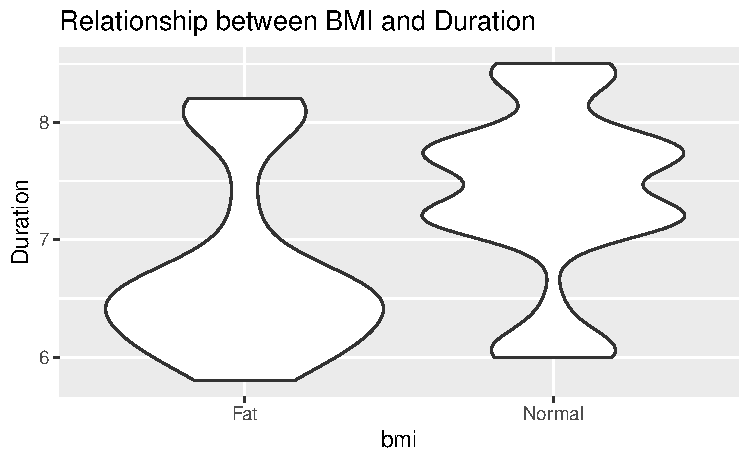
\includegraphics[width=0.7\linewidth]{SleepHelath_files/figure-latex/unnamed-chunk-22-1} \end{center}

\hypertarget{box-plot}{%
\subsection{Box plot}\label{box-plot}}

\begin{Shaded}
\begin{Highlighting}[]
\NormalTok{Sleep\_health\_and\_lifestyle\_dataset\_renamed }\SpecialCharTok{\%\textgreater{}\%}
  \FunctionTok{ggplot}\NormalTok{() }\SpecialCharTok{+}
    \FunctionTok{geom\_boxplot}\NormalTok{(}\AttributeTok{mapping =} \FunctionTok{aes}\NormalTok{(}\AttributeTok{x =}\NormalTok{ HRate)) }\SpecialCharTok{+}
    \FunctionTok{labs}\NormalTok{(}\AttributeTok{title =} \StringTok{"Boxplot of Individual Heart Rate"}\NormalTok{, }\AttributeTok{x =} \StringTok{"Heart rate"}\NormalTok{)}
\end{Highlighting}
\end{Shaded}

\begin{center}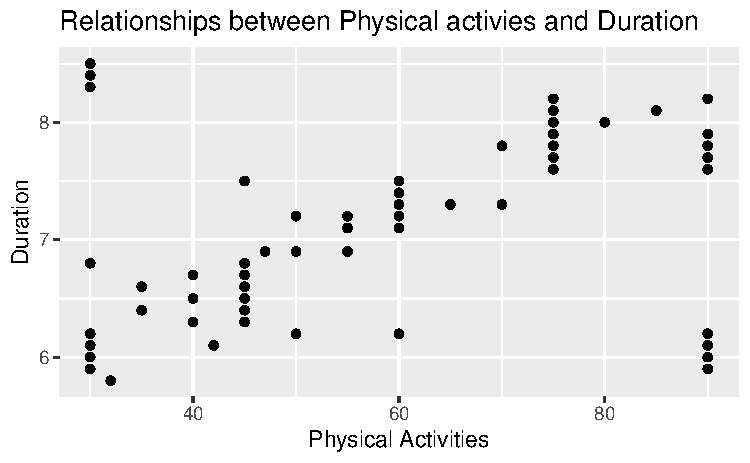
\includegraphics[width=0.7\linewidth]{SleepHelath_files/figure-latex/unnamed-chunk-23-1} \end{center}

\hypertarget{violin-plot}{%
\subsection{Violin plot}\label{violin-plot}}

\begin{Shaded}
\begin{Highlighting}[]
\NormalTok{Sleep\_health\_and\_lifestyle\_dataset\_renamed }\SpecialCharTok{\%\textgreater{}\%}
  \FunctionTok{ggplot}\NormalTok{() }\SpecialCharTok{+}
    \FunctionTok{geom\_violin}\NormalTok{(}\AttributeTok{mapping =} \FunctionTok{aes}\NormalTok{(}\AttributeTok{x =}\NormalTok{ HRate, }\AttributeTok{y =}\StringTok{""}\NormalTok{)) }\SpecialCharTok{+}
    \FunctionTok{labs}\NormalTok{(}\AttributeTok{title =} \StringTok{"Violin of Individual Heart rate"}\NormalTok{, }\AttributeTok{x =} \StringTok{"Heart rate"}\NormalTok{, }\AttributeTok{y =} \StringTok{"y"}\NormalTok{)}
\end{Highlighting}
\end{Shaded}

\begin{center}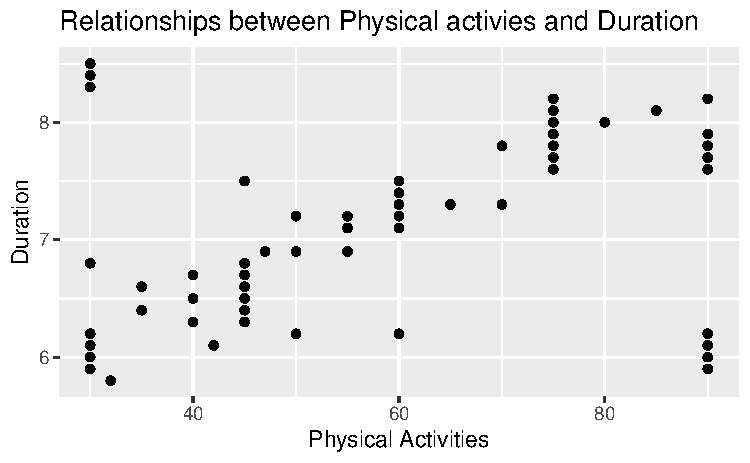
\includegraphics[width=0.7\linewidth]{SleepHelath_files/figure-latex/unnamed-chunk-24-1} \end{center}

\begin{Shaded}
\begin{Highlighting}[]
\NormalTok{Sleep\_health\_and\_lifestyle\_dataset\_renamed }\SpecialCharTok{\%\textgreater{}\%}
  \FunctionTok{ggplot}\NormalTok{() }\SpecialCharTok{+}
  \FunctionTok{geom\_bin2d}\NormalTok{(}\AttributeTok{mapping =} \FunctionTok{aes}\NormalTok{(}\AttributeTok{x =}\NormalTok{ HRate, }\AttributeTok{y =}\NormalTok{ Duration)) }\SpecialCharTok{+}
  \FunctionTok{labs}\NormalTok{(}\AttributeTok{title =} \StringTok{"HRate and Duration "}\NormalTok{,}\AttributeTok{x =} \StringTok{"Heart Rate"}\NormalTok{,}\AttributeTok{y =} \StringTok{"Duration"}\NormalTok{) }\SpecialCharTok{+} \FunctionTok{scale\_fill\_viridis\_c}\NormalTok{(}\AttributeTok{trans =} \StringTok{"log"}\NormalTok{)}
\end{Highlighting}
\end{Shaded}

\begin{center}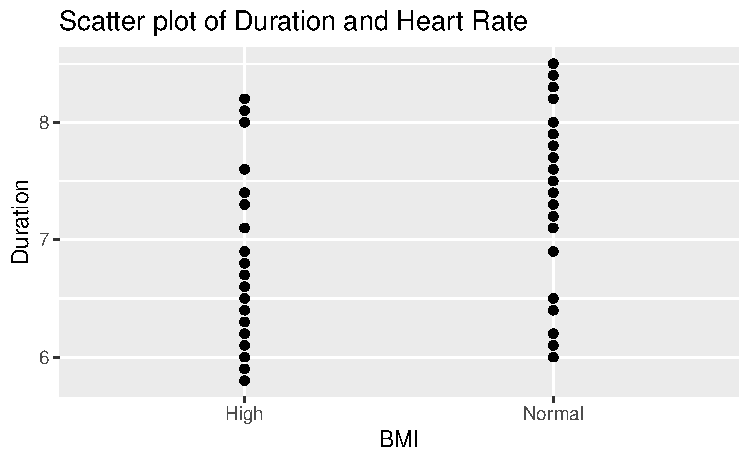
\includegraphics[width=0.7\linewidth]{SleepHelath_files/figure-latex/unnamed-chunk-25-1} \end{center}

\hypertarget{bar-graph}{%
\subsection{Bar Graph}\label{bar-graph}}

\begin{Shaded}
\begin{Highlighting}[]
\NormalTok{Sleep\_health\_and\_lifestyle\_dataset\_renamed }\SpecialCharTok{\%\textgreater{}\%}
  \FunctionTok{ggplot}\NormalTok{() }\SpecialCharTok{+}
    \FunctionTok{geom\_bar}\NormalTok{(}\AttributeTok{mapping =} \FunctionTok{aes}\NormalTok{(}\AttributeTok{x =}\NormalTok{ BMI)) }\SpecialCharTok{+}
    \FunctionTok{labs}\NormalTok{(}\AttributeTok{title =} \StringTok{"BMI Count"}\NormalTok{, }\AttributeTok{x =} \StringTok{"BMI"}\NormalTok{)}
\end{Highlighting}
\end{Shaded}

\begin{center}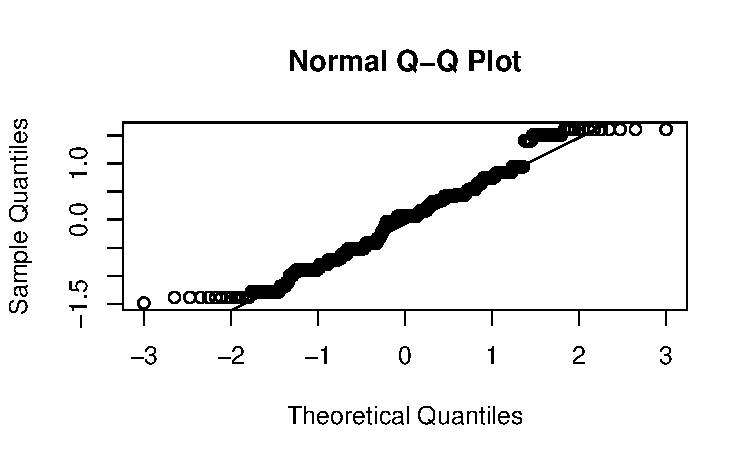
\includegraphics[width=0.7\linewidth]{SleepHelath_files/figure-latex/unnamed-chunk-26-1} \end{center}

\hypertarget{box-plot-1}{%
\subsection{Box plot}\label{box-plot-1}}

\begin{Shaded}
\begin{Highlighting}[]
\NormalTok{Sleep\_health\_and\_lifestyle\_dataset\_renamed }\SpecialCharTok{\%\textgreater{}\%}
  \FunctionTok{ggplot}\NormalTok{() }\SpecialCharTok{+}
    \FunctionTok{geom\_boxplot}\NormalTok{(}\AttributeTok{mapping =} \FunctionTok{aes}\NormalTok{(}\AttributeTok{x =}\NormalTok{ BMI, }\AttributeTok{y =}\NormalTok{ Duration)) }\SpecialCharTok{+}
    \FunctionTok{labs}\NormalTok{(}\AttributeTok{title =} \StringTok{"Relationship between BMI and Duration"}\NormalTok{, }\AttributeTok{x =} \StringTok{"BMI"}\NormalTok{)}
\end{Highlighting}
\end{Shaded}

\begin{center}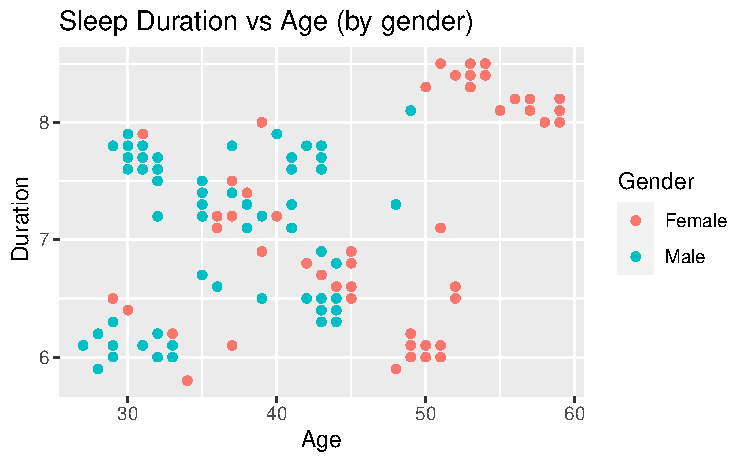
\includegraphics[width=0.7\linewidth]{SleepHelath_files/figure-latex/unnamed-chunk-27-1} \end{center}

\hypertarget{violin-plot-1}{%
\subsection{Violin plot}\label{violin-plot-1}}

\begin{Shaded}
\begin{Highlighting}[]
\NormalTok{Sleep\_health\_and\_lifestyle\_dataset\_renamed }\SpecialCharTok{\%\textgreater{}\%}
  \FunctionTok{ggplot}\NormalTok{() }\SpecialCharTok{+}
    \FunctionTok{geom\_violin}\NormalTok{(}\AttributeTok{mapping =} \FunctionTok{aes}\NormalTok{(}\AttributeTok{x =}\NormalTok{ BMI, }\AttributeTok{y =}\NormalTok{ Duration)) }\SpecialCharTok{+}
    \FunctionTok{labs}\NormalTok{(}\AttributeTok{title =} \StringTok{"Relationship between BMI and Duration"}\NormalTok{, }\AttributeTok{x =} \StringTok{"bmi"}\NormalTok{, }\AttributeTok{y =} \StringTok{"Duration"}\NormalTok{)}
\end{Highlighting}
\end{Shaded}

\begin{center}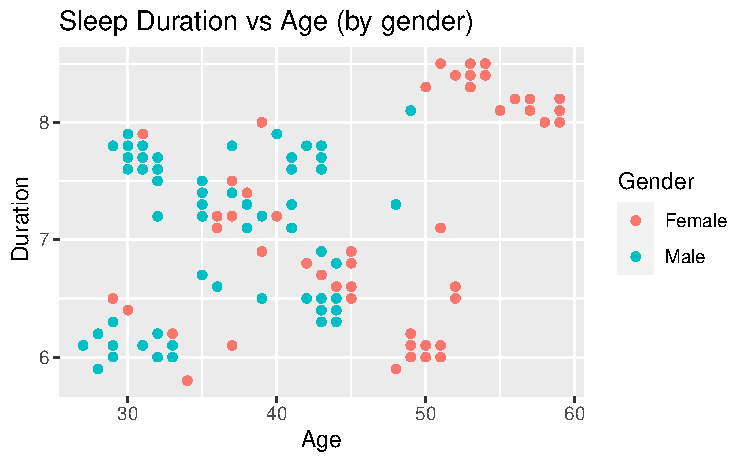
\includegraphics[width=0.7\linewidth]{SleepHelath_files/figure-latex/unnamed-chunk-28-1} \end{center}

\#Scatter plot\_Duration and Heart Rate

\begin{Shaded}
\begin{Highlighting}[]
\NormalTok{Sleep\_health\_and\_lifestyle\_dataset\_renamed    }\SpecialCharTok{\%\textgreater{}\%} 
\FunctionTok{ggplot}\NormalTok{()    }\SpecialCharTok{+}
\FunctionTok{geom\_point}\NormalTok{(}\AttributeTok{mapping =} \FunctionTok{aes}\NormalTok{(}\AttributeTok{x =}\NormalTok{ BMI, }\AttributeTok{y =}\NormalTok{ Duration))    }\SpecialCharTok{+} 
\FunctionTok{labs}\NormalTok{(}
\AttributeTok{title =} \StringTok{"Scatter plot of Duration and Heart Rate"}\NormalTok{, }
\AttributeTok{x =} \StringTok{"BMI"}\NormalTok{,}
\AttributeTok{y =} \StringTok{"Duration"} 
\NormalTok{)}
\end{Highlighting}
\end{Shaded}

\begin{center}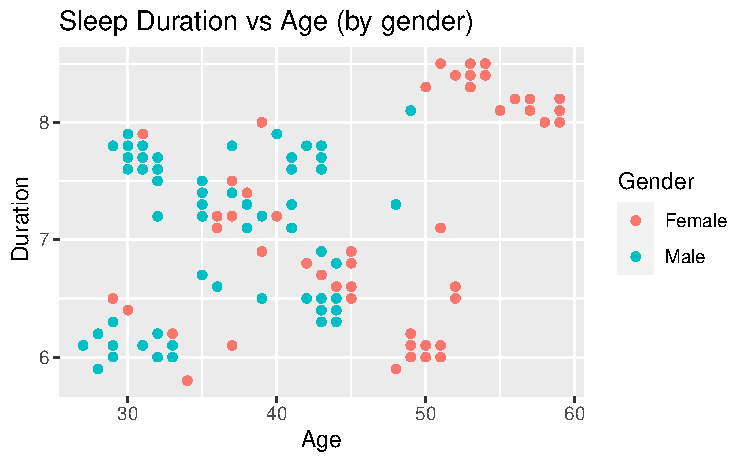
\includegraphics[width=0.7\linewidth]{SleepHelath_files/figure-latex/unnamed-chunk-29-1} \end{center}

\hypertarget{part-5-_-modeling}{%
\subsubsection{PART 5 \_ Modeling}\label{part-5-_-modeling}}

\begin{Shaded}
\begin{Highlighting}[]
\NormalTok{Sleep\_health\_and\_lifestyle\_dataset\_renamed}\SpecialCharTok{\%\textgreater{}\%}
  \FunctionTok{ggplot}\NormalTok{()}\SpecialCharTok{+}
  \FunctionTok{geom\_point}\NormalTok{( }\AttributeTok{mapping =} \FunctionTok{aes}\NormalTok{( }\AttributeTok{x  =}\NormalTok{ Physical , }\AttributeTok{y =}\NormalTok{ Duration)) }\SpecialCharTok{+}
  \FunctionTok{labs}\NormalTok{(}\AttributeTok{title =} \StringTok{"Relationships between Physical activies and Duration"}\NormalTok{,}
       \AttributeTok{x =} \StringTok{"Physical Activities"}\NormalTok{ , }\AttributeTok{y =} \StringTok{"Duration"}\NormalTok{)}
\end{Highlighting}
\end{Shaded}

\begin{center}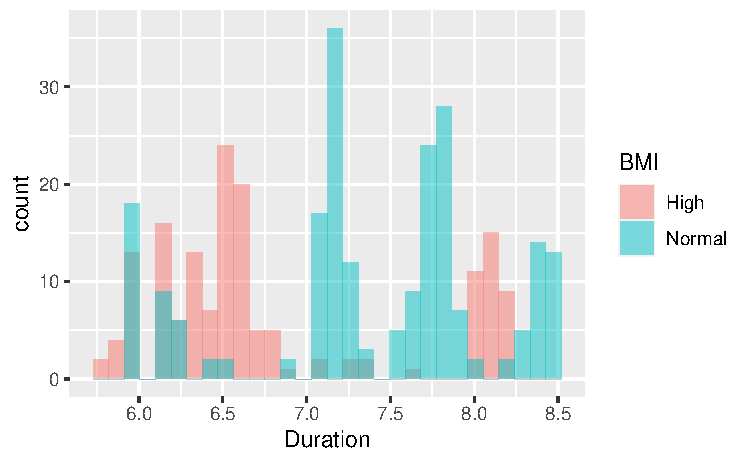
\includegraphics[width=0.7\linewidth]{SleepHelath_files/figure-latex/unnamed-chunk-30-1} \end{center}

\begin{Shaded}
\begin{Highlighting}[]
\NormalTok{data }\OtherTok{\textless{}{-}}\NormalTok{ Sleep\_health\_and\_lifestyle\_dataset\_renamed}

\NormalTok{model }\OtherTok{\textless{}{-}} \FunctionTok{lm}\NormalTok{(Duration }\SpecialCharTok{\textasciitilde{}}\NormalTok{ Physical, }\AttributeTok{data =}\NormalTok{ Sleep\_health\_and\_lifestyle\_dataset\_renamed)}


\FunctionTok{summary}\NormalTok{(model)}
\end{Highlighting}
\end{Shaded}

\begin{verbatim}
## 
## Call:
## lm(formula = Duration ~ Physical, data = Sleep_health_and_lifestyle_dataset_renamed)
## 
## Residuals:
##      Min       1Q   Median       3Q      Max 
## -1.48215 -0.59686  0.06119  0.43952  1.60453 
## 
## Coefficients:
##             Estimate Std. Error t value Pr(>|t|)    
## (Intercept) 6.652128   0.121379  54.805  < 2e-16 ***
## Physical    0.008111   0.001935   4.191 3.47e-05 ***
## ---
## Signif. codes:  0 '***' 0.001 '**' 0.01 '*' 0.05 '.' 0.1 ' ' 1
## 
## Residual standard error: 0.7786 on 372 degrees of freedom
## Multiple R-squared:  0.0451, Adjusted R-squared:  0.04253 
## F-statistic: 17.57 on 1 and 372 DF,  p-value: 3.467e-05
\end{verbatim}

\begin{Shaded}
\begin{Highlighting}[]
\NormalTok{residuals }\OtherTok{\textless{}{-}} \FunctionTok{residuals}\NormalTok{(model)}

\FunctionTok{qqnorm}\NormalTok{(residuals)}
\FunctionTok{qqline}\NormalTok{(residuals)}
\end{Highlighting}
\end{Shaded}

\begin{center}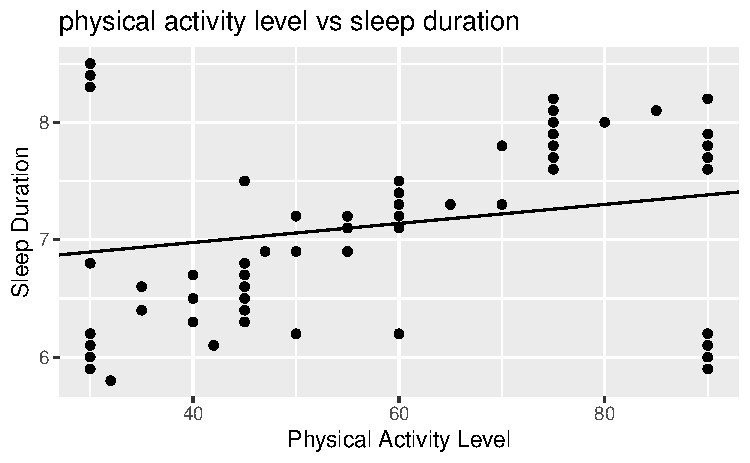
\includegraphics[width=0.7\linewidth]{SleepHelath_files/figure-latex/unnamed-chunk-32-1} \end{center}

\begin{Shaded}
\begin{Highlighting}[]
\FunctionTok{labs}\NormalTok{( }\AttributeTok{title  =} \StringTok{"QQplot"}\NormalTok{ , }\AttributeTok{x =} \StringTok{"Theoretical"}\NormalTok{ , }\AttributeTok{y =} \StringTok{"Quantaties"}\NormalTok{)}
\end{Highlighting}
\end{Shaded}

\begin{verbatim}
## $x
## [1] "Theoretical"
## 
## $y
## [1] "Quantaties"
## 
## $title
## [1] "QQplot"
## 
## attr(,"class")
## [1] "labels"
\end{verbatim}

\begin{Shaded}
\begin{Highlighting}[]
\NormalTok{Renamed\_other\_model }\OtherTok{\textless{}{-}} \FunctionTok{lm}\NormalTok{(Duration }\SpecialCharTok{\textasciitilde{}}\NormalTok{ Physical, }\AttributeTok{data =}\NormalTok{ Sleep\_health\_and\_lifestyle\_dataset\_renamed)}
\end{Highlighting}
\end{Shaded}

\begin{Shaded}
\begin{Highlighting}[]
\NormalTok{Renamed\_other\_model}\SpecialCharTok{$}\NormalTok{coefficients}
\end{Highlighting}
\end{Shaded}

\begin{verbatim}
## (Intercept)    Physical 
## 6.652127945 0.008111349
\end{verbatim}

\begin{Shaded}
\begin{Highlighting}[]
\NormalTok{Renamed\_other\_model}\SpecialCharTok{\%\textgreater{}\%}
  \FunctionTok{tidy}\NormalTok{()}
\end{Highlighting}
\end{Shaded}

\begin{longtable}[]{@{}lrrrr@{}}
\toprule\noalign{}
term & estimate & std.error & statistic & p.value \\
\midrule\noalign{}
\endhead
\bottomrule\noalign{}
\endlastfoot
(Intercept) & 6.6521279 & 0.1213792 & 54.804523 & 0.00e+00 \\
Physical & 0.0081113 & 0.0019352 & 4.191459 & 3.47e-05 \\
\end{longtable}

\begin{Shaded}
\begin{Highlighting}[]
\NormalTok{Renamed\_other\_model}\SpecialCharTok{\%\textgreater{}\%}
  \FunctionTok{glance}\NormalTok{()}\SpecialCharTok{\%\textgreater{}\%}
  \FunctionTok{select}\NormalTok{(r.squared)}
\end{Highlighting}
\end{Shaded}

\begin{longtable}[]{@{}r@{}}
\toprule\noalign{}
r.squared \\
\midrule\noalign{}
\endhead
\bottomrule\noalign{}
\endlastfoot
0.0450969 \\
\end{longtable}

\begin{Shaded}
\begin{Highlighting}[]
\NormalTok{Sleep\_health\_and\_lifestyle\_dataset\_renamed}\SpecialCharTok{\%\textgreater{}\%}
  \FunctionTok{ggplot}\NormalTok{()}\SpecialCharTok{+}
  \FunctionTok{geom\_point}\NormalTok{(}\AttributeTok{mapping =} \FunctionTok{aes}\NormalTok{( }\AttributeTok{x  =}\NormalTok{ Physical , }\AttributeTok{y =}\NormalTok{ Duration) )}\SpecialCharTok{+}
  \FunctionTok{geom\_abline}\NormalTok{(}\AttributeTok{slope =}\NormalTok{ Renamed\_other\_model}\SpecialCharTok{$}\NormalTok{coefficients[}\DecValTok{2}\NormalTok{]   ,}
              \AttributeTok{intercept =}\NormalTok{ Renamed\_other\_model}\SpecialCharTok{$}\NormalTok{coefficients[}\DecValTok{1}\NormalTok{]  )}\SpecialCharTok{+}
  \FunctionTok{labs}\NormalTok{( }\AttributeTok{title =} \StringTok{"Relationships between Physical and Duration"}\NormalTok{,}
        \AttributeTok{x =} \StringTok{" Physical "}\NormalTok{,}
        \AttributeTok{y =} \StringTok{" Duration"}\NormalTok{ )}
\end{Highlighting}
\end{Shaded}

\begin{center}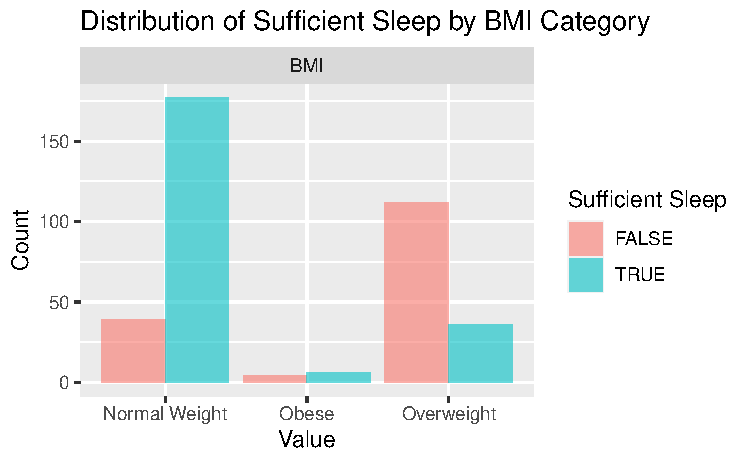
\includegraphics[width=0.7\linewidth]{SleepHelath_files/figure-latex/unnamed-chunk-37-1} \end{center}

\#\#\#Part 9

\begin{Shaded}
\begin{Highlighting}[]
\FunctionTok{library}\NormalTok{(tidyr)}
\FunctionTok{library}\NormalTok{(ggplot2)}
\FunctionTok{library}\NormalTok{(dplyr)}
\FunctionTok{library}\NormalTok{(readr)}
\FunctionTok{library}\NormalTok{(class)}
\FunctionTok{library}\NormalTok{(caret)}

\NormalTok{Sleep\_health\_and\_lifestyle\_dataset }\OtherTok{\textless{}{-}} \FunctionTok{read\_csv}\NormalTok{(}\AttributeTok{file =} \StringTok{"Sleep\_health\_and\_lifestyle\_dataset.csv"}\NormalTok{,}
  \AttributeTok{col\_types =} \FunctionTok{cols}\NormalTok{(}
    \StringTok{\textquotesingle{}Person ID\textquotesingle{}} \OtherTok{=} \FunctionTok{col\_character}\NormalTok{(),}
    \StringTok{\textquotesingle{}Age\textquotesingle{}} \OtherTok{=} \FunctionTok{col\_double}\NormalTok{(),}
    \StringTok{\textquotesingle{}Sleep Duration\textquotesingle{}} \OtherTok{=} \FunctionTok{col\_double}\NormalTok{(),}
    \StringTok{\textquotesingle{}Stress Level\textquotesingle{}} \OtherTok{=} \FunctionTok{col\_double}\NormalTok{(),}
    \StringTok{\textquotesingle{}Physical Activity Level\textquotesingle{}} \OtherTok{=} \FunctionTok{col\_double}\NormalTok{(),}
    \StringTok{\textquotesingle{}Quality of Sleep\textquotesingle{}} \OtherTok{=} \FunctionTok{col\_double}\NormalTok{(),}
    \StringTok{\textquotesingle{}BMI Category\textquotesingle{}} \OtherTok{=} \FunctionTok{col\_character}\NormalTok{(),}
    \StringTok{\textquotesingle{}Blood Pressure\textquotesingle{}} \OtherTok{=} \FunctionTok{col\_character}\NormalTok{(),}
    \StringTok{\textquotesingle{}Heart Rate\textquotesingle{}} \OtherTok{=} \FunctionTok{col\_double}\NormalTok{(),}
    \StringTok{\textquotesingle{}Daily Steps\textquotesingle{}} \OtherTok{=} \FunctionTok{col\_double}\NormalTok{(),}
    \StringTok{\textquotesingle{}Sleep Disorder\textquotesingle{}} \OtherTok{=} \FunctionTok{col\_character}\NormalTok{()}
\NormalTok{  ))}

\NormalTok{Sleep\_health\_and\_lifestyle\_dataset\_renamed }\OtherTok{\textless{}{-}}\NormalTok{ Sleep\_health\_and\_lifestyle\_dataset }\SpecialCharTok{\%\textgreater{}\%}
  \FunctionTok{rename}\NormalTok{(}\AttributeTok{ID =} \StringTok{\textquotesingle{}Person ID\textquotesingle{}}\NormalTok{,}
         \AttributeTok{Duration =} \StringTok{\textquotesingle{}Sleep Duration\textquotesingle{}}\NormalTok{,}
         \AttributeTok{Stress =} \StringTok{\textquotesingle{}Stress Level\textquotesingle{}}\NormalTok{,}
         \AttributeTok{Physical =} \StringTok{\textquotesingle{}Physical Activity Level\textquotesingle{}}\NormalTok{,}
         \AttributeTok{Quality =} \StringTok{\textquotesingle{}Quality of Sleep\textquotesingle{}}\NormalTok{,}
         \AttributeTok{BMI =} \StringTok{\textquotesingle{}BMI Category\textquotesingle{}}\NormalTok{,}
         \AttributeTok{BPressure =} \StringTok{\textquotesingle{}Blood Pressure\textquotesingle{}}\NormalTok{,}
         \AttributeTok{HRate =} \StringTok{\textquotesingle{}Heart Rate\textquotesingle{}}\NormalTok{,}
         \AttributeTok{DSteps =} \StringTok{\textquotesingle{}Daily Steps\textquotesingle{}}\NormalTok{,}
         \AttributeTok{Disorder =} \StringTok{\textquotesingle{}Sleep Disorder\textquotesingle{}}\NormalTok{)}


\NormalTok{sleep\_data }\OtherTok{\textless{}{-}}\NormalTok{ Sleep\_health\_and\_lifestyle\_dataset\_renamed }\SpecialCharTok{\%\textgreater{}\%}
    \FunctionTok{mutate}\NormalTok{(}\AttributeTok{sufficient\_sleep =}\NormalTok{ Duration }\SpecialCharTok{\textgreater{}=} \FloatTok{7.0}\NormalTok{)}
\end{Highlighting}
\end{Shaded}

\begin{Shaded}
\begin{Highlighting}[]
\NormalTok{sleep\_data }\SpecialCharTok{\%\textgreater{}\%}
  \FunctionTok{pivot\_longer}\NormalTok{(}\AttributeTok{cols =} \FunctionTok{c}\NormalTok{(Disorder), }\AttributeTok{names\_to =} \StringTok{"variable"}\NormalTok{, }\AttributeTok{values\_to =} \StringTok{"value"}\NormalTok{) }\SpecialCharTok{\%\textgreater{}\%}
  \FunctionTok{group\_by}\NormalTok{(variable, value, sufficient\_sleep) }\SpecialCharTok{\%\textgreater{}\%}
  \FunctionTok{summarise}\NormalTok{(}\AttributeTok{count =} \FunctionTok{n}\NormalTok{()) }\SpecialCharTok{\%\textgreater{}\%}
  \FunctionTok{ggplot}\NormalTok{() }\SpecialCharTok{+}
  \FunctionTok{geom\_bar}\NormalTok{(}
    \AttributeTok{mapping =} \FunctionTok{aes}\NormalTok{(}\AttributeTok{x =}\NormalTok{ value, }\AttributeTok{y =}\NormalTok{ count, }\AttributeTok{fill =}\NormalTok{ sufficient\_sleep),}
    \AttributeTok{position =} \StringTok{"dodge"}\NormalTok{,   }
    \AttributeTok{alpha =} \FloatTok{0.6}\NormalTok{,}
    \AttributeTok{stat =} \StringTok{"identity"}
\NormalTok{  ) }\SpecialCharTok{+}
  \FunctionTok{facet\_wrap}\NormalTok{(}\SpecialCharTok{\textasciitilde{}}\NormalTok{ variable, }\AttributeTok{scales =} \StringTok{"free"}\NormalTok{) }\SpecialCharTok{+}
  \FunctionTok{labs}\NormalTok{(}\AttributeTok{title =} \StringTok{"Distribution of Sufficient Sleep across Disorders"}\NormalTok{,}
       \AttributeTok{x =} \StringTok{"Disorder Type"}\NormalTok{, }
       \AttributeTok{y =} \StringTok{"Count"}\NormalTok{, }
       \AttributeTok{fill =} \StringTok{"Sufficient Sleep"}\NormalTok{)}
\end{Highlighting}
\end{Shaded}

\begin{verbatim}
## `summarise()` has grouped output by 'variable', 'value'. You can override using
## the `.groups` argument.
\end{verbatim}

\begin{center}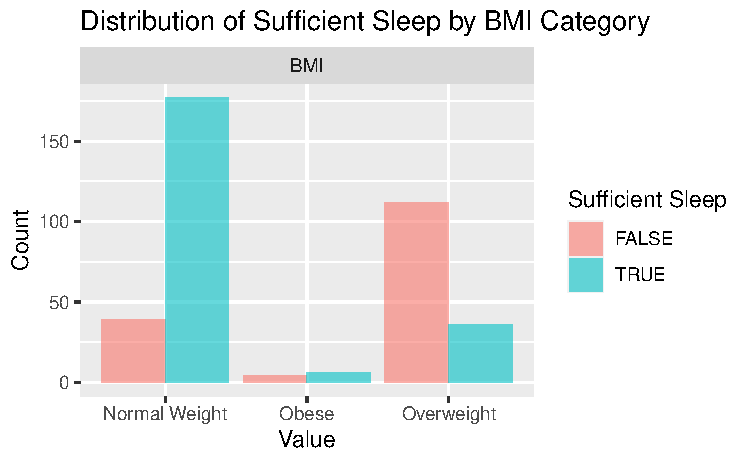
\includegraphics[width=0.7\linewidth]{SleepHelath_files/figure-latex/unnamed-chunk-39-1} \end{center}

\begin{Shaded}
\begin{Highlighting}[]
\NormalTok{sleep\_data }\SpecialCharTok{\%\textgreater{}\%}
  \FunctionTok{pivot\_longer}\NormalTok{(}\AttributeTok{cols =} \FunctionTok{c}\NormalTok{(Gender), }\AttributeTok{names\_to =} \StringTok{"variable"}\NormalTok{, }\AttributeTok{values\_to =} \StringTok{"value"}\NormalTok{) }\SpecialCharTok{\%\textgreater{}\%}
  \FunctionTok{group\_by}\NormalTok{(variable, value, sufficient\_sleep) }\SpecialCharTok{\%\textgreater{}\%}
  \FunctionTok{summarise}\NormalTok{(}\AttributeTok{count =} \FunctionTok{n}\NormalTok{()) }\SpecialCharTok{\%\textgreater{}\%}
  \FunctionTok{ggplot}\NormalTok{() }\SpecialCharTok{+}
  \FunctionTok{geom\_bar}\NormalTok{(}
    \AttributeTok{mapping =} \FunctionTok{aes}\NormalTok{(}\AttributeTok{x =}\NormalTok{ value, }\AttributeTok{y =}\NormalTok{ count, }\AttributeTok{fill =}\NormalTok{ sufficient\_sleep),}
    \AttributeTok{position =} \StringTok{"dodge"}\NormalTok{,  }
    \AttributeTok{alpha =} \FloatTok{0.6}\NormalTok{,}
    \AttributeTok{stat =} \StringTok{"identity"}
\NormalTok{  ) }\SpecialCharTok{+}
  \FunctionTok{facet\_wrap}\NormalTok{(}\SpecialCharTok{\textasciitilde{}}\NormalTok{ variable, }\AttributeTok{scales =} \StringTok{"free"}\NormalTok{) }\SpecialCharTok{+}
  \FunctionTok{labs}\NormalTok{(}\AttributeTok{title =} \StringTok{"Distribution of Sufficient Sleep by Gender"}\NormalTok{,}
       \AttributeTok{x =} \StringTok{"Value"}\NormalTok{, }
       \AttributeTok{y =} \StringTok{"Count"}\NormalTok{, }
       \AttributeTok{fill =} \StringTok{"Sufficient Sleep"}\NormalTok{)}
\end{Highlighting}
\end{Shaded}

\begin{verbatim}
## `summarise()` has grouped output by 'variable', 'value'. You can override using
## the `.groups` argument.
\end{verbatim}

\begin{center}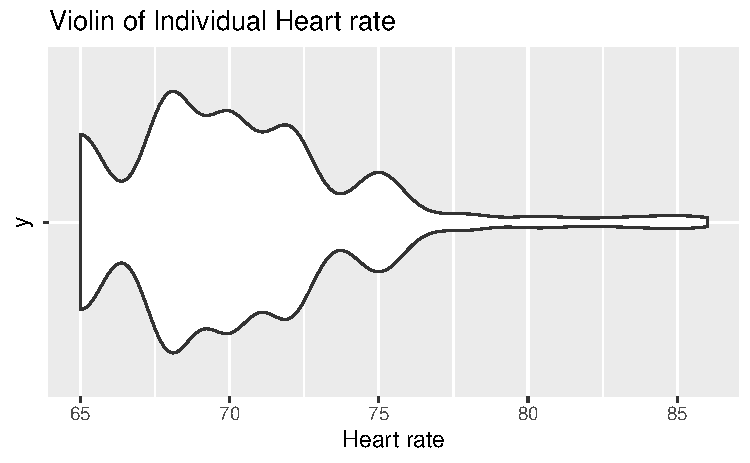
\includegraphics[width=0.7\linewidth]{SleepHelath_files/figure-latex/unnamed-chunk-40-1} \end{center}

\begin{Shaded}
\begin{Highlighting}[]
\NormalTok{sleep\_data }\SpecialCharTok{\%\textgreater{}\%}
  \FunctionTok{pivot\_longer}\NormalTok{(}\AttributeTok{cols =} \FunctionTok{c}\NormalTok{(BMI), }\AttributeTok{names\_to =} \StringTok{"variable"}\NormalTok{, }\AttributeTok{values\_to =} \StringTok{"value"}\NormalTok{) }\SpecialCharTok{\%\textgreater{}\%}
  \FunctionTok{mutate}\NormalTok{(}\AttributeTok{value =} \FunctionTok{ifelse}\NormalTok{(value }\SpecialCharTok{==} \StringTok{"Normal"}\NormalTok{, }\StringTok{"Normal Weight"}\NormalTok{, value)) }\SpecialCharTok{\%\textgreater{}\%}
  \FunctionTok{group\_by}\NormalTok{(variable, value, sufficient\_sleep) }\SpecialCharTok{\%\textgreater{}\%}
  \FunctionTok{summarise}\NormalTok{(}\AttributeTok{count =} \FunctionTok{n}\NormalTok{()) }\SpecialCharTok{\%\textgreater{}\%}
  \FunctionTok{ggplot}\NormalTok{() }\SpecialCharTok{+}
  \FunctionTok{geom\_bar}\NormalTok{(}
    \AttributeTok{mapping =} \FunctionTok{aes}\NormalTok{(}\AttributeTok{x =}\NormalTok{ value, }\AttributeTok{y =}\NormalTok{ count, }\AttributeTok{fill =}\NormalTok{ sufficient\_sleep),}
    \AttributeTok{position =} \StringTok{"dodge"}\NormalTok{,   }
    \AttributeTok{alpha =} \FloatTok{0.6}\NormalTok{,}
    \AttributeTok{stat =} \StringTok{"identity"}
\NormalTok{  ) }\SpecialCharTok{+}
  \FunctionTok{facet\_wrap}\NormalTok{(}\SpecialCharTok{\textasciitilde{}}\NormalTok{ variable, }\AttributeTok{scales =} \StringTok{"free"}\NormalTok{) }\SpecialCharTok{+}
  \FunctionTok{labs}\NormalTok{(}\AttributeTok{title =} \StringTok{"Distribution of Sufficient Sleep by BMI Category"}\NormalTok{,}
       \AttributeTok{x =} \StringTok{"Value"}\NormalTok{, }
       \AttributeTok{y =} \StringTok{"Count"}\NormalTok{, }
       \AttributeTok{fill =} \StringTok{"Sufficient Sleep"}\NormalTok{)}
\end{Highlighting}
\end{Shaded}

\begin{verbatim}
## `summarise()` has grouped output by 'variable', 'value'. You can override using
## the `.groups` argument.
\end{verbatim}

\begin{center}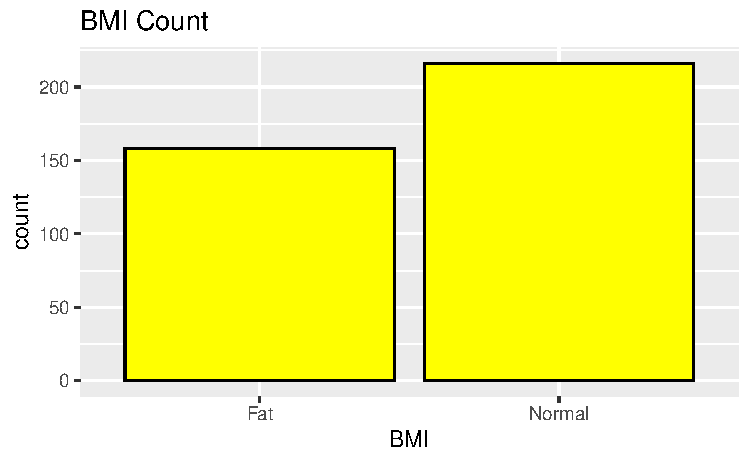
\includegraphics[width=0.7\linewidth]{SleepHelath_files/figure-latex/unnamed-chunk-41-1} \end{center}

\begin{Shaded}
\begin{Highlighting}[]
\NormalTok{sleep\_data }\SpecialCharTok{\%\textgreater{}\%}
  \FunctionTok{pivot\_longer}\NormalTok{(}\AttributeTok{cols =} \FunctionTok{c}\NormalTok{(BMI), }\AttributeTok{names\_to =} \StringTok{"variable"}\NormalTok{, }\AttributeTok{values\_to =} \StringTok{"value"}\NormalTok{) }\SpecialCharTok{\%\textgreater{}\%}
  \FunctionTok{mutate}\NormalTok{(}\AttributeTok{value =} \FunctionTok{ifelse}\NormalTok{(value }\SpecialCharTok{==} \StringTok{"Normal"}\NormalTok{, }\StringTok{"Normal Weight"}\NormalTok{, value)) }\SpecialCharTok{\%\textgreater{}\%}
  \FunctionTok{group\_by}\NormalTok{(variable, value, sufficient\_sleep) }\SpecialCharTok{\%\textgreater{}\%}
  \FunctionTok{summarise}\NormalTok{(}\AttributeTok{count =} \FunctionTok{n}\NormalTok{()) }\SpecialCharTok{\%\textgreater{}\%}
  \FunctionTok{ggplot}\NormalTok{() }\SpecialCharTok{+}
  \FunctionTok{geom\_bar}\NormalTok{(}
    \AttributeTok{mapping =} \FunctionTok{aes}\NormalTok{(}\AttributeTok{x =}\NormalTok{ value, }\AttributeTok{y =}\NormalTok{ count, }\AttributeTok{fill =}\NormalTok{ sufficient\_sleep),}
    \AttributeTok{position =} \StringTok{"dodge"}\NormalTok{,   }
    \AttributeTok{alpha =} \FloatTok{0.6}\NormalTok{,}
    \AttributeTok{stat =} \StringTok{"identity"}
\NormalTok{  ) }\SpecialCharTok{+}
  \FunctionTok{facet\_wrap}\NormalTok{(}\SpecialCharTok{\textasciitilde{}}\NormalTok{ variable, }\AttributeTok{scales =} \StringTok{"free"}\NormalTok{) }\SpecialCharTok{+}
  \FunctionTok{labs}\NormalTok{(}\AttributeTok{title =} \StringTok{"Distribution of Sufficient Sleep by BMI Category"}\NormalTok{,}
       \AttributeTok{x =} \StringTok{"Value"}\NormalTok{, }
       \AttributeTok{y =} \StringTok{"Count"}\NormalTok{, }
       \AttributeTok{fill =} \StringTok{"Sufficient Sleep"}\NormalTok{)}
\end{Highlighting}
\end{Shaded}

\begin{verbatim}
## `summarise()` has grouped output by 'variable', 'value'. You can override using
## the `.groups` argument.
\end{verbatim}

\begin{center}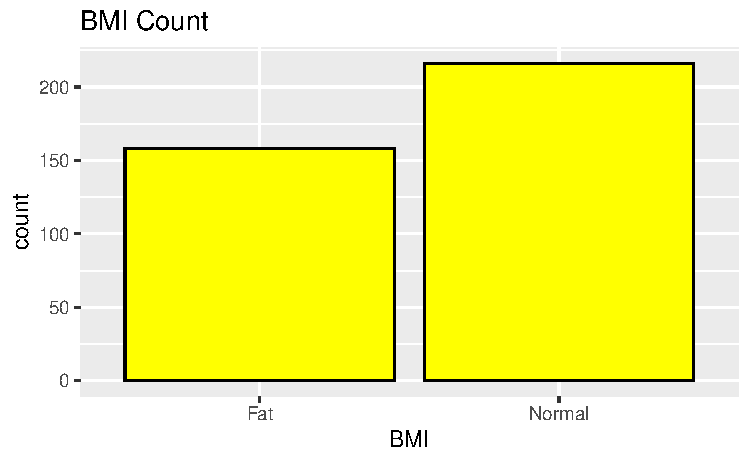
\includegraphics[width=0.7\linewidth]{SleepHelath_files/figure-latex/unnamed-chunk-42-1} \end{center}

\begin{Shaded}
\begin{Highlighting}[]
\NormalTok{mode\_gender }\OtherTok{\textless{}{-}} \FunctionTok{as.character}\NormalTok{(}\FunctionTok{names}\NormalTok{(}\FunctionTok{which.max}\NormalTok{(}\FunctionTok{table}\NormalTok{(sleep\_data}\SpecialCharTok{$}\NormalTok{Gender))))}
\NormalTok{mode\_occupation }\OtherTok{\textless{}{-}} \FunctionTok{as.character}\NormalTok{(}\FunctionTok{names}\NormalTok{(}\FunctionTok{which.max}\NormalTok{(}\FunctionTok{table}\NormalTok{(sleep\_data}\SpecialCharTok{$}\NormalTok{Occupation))))}
\NormalTok{mode\_bmi }\OtherTok{\textless{}{-}} \FunctionTok{as.character}\NormalTok{(}\FunctionTok{names}\NormalTok{(}\FunctionTok{which.max}\NormalTok{(}\FunctionTok{table}\NormalTok{(sleep\_data}\SpecialCharTok{$}\NormalTok{BMI))))}

\NormalTok{sleep\_data }\OtherTok{\textless{}{-}}\NormalTok{ sleep\_data }\SpecialCharTok{\%\textgreater{}\%}
\FunctionTok{mutate}\NormalTok{(}
  \AttributeTok{Gender =} \FunctionTok{if\_else}\NormalTok{(}\FunctionTok{is.na}\NormalTok{(Gender), mode\_gender, Gender),}
  \AttributeTok{Occupation =} \FunctionTok{if\_else}\NormalTok{(}\FunctionTok{is.na}\NormalTok{(Occupation), mode\_occupation, Occupation),}
  \AttributeTok{BMI =} \FunctionTok{if\_else}\NormalTok{(}\FunctionTok{is.na}\NormalTok{(BMI), mode\_bmi, BMI)}
\NormalTok{)}
\end{Highlighting}
\end{Shaded}

\begin{Shaded}
\begin{Highlighting}[]
\NormalTok{sleep\_data}\SpecialCharTok{$}\NormalTok{sufficient\_sleep }\OtherTok{\textless{}{-}} \FunctionTok{ifelse}\NormalTok{(sleep\_data}\SpecialCharTok{$}\NormalTok{Duration }\SpecialCharTok{\textgreater{}=} \DecValTok{7}\NormalTok{, }\StringTok{"Sufficient"}\NormalTok{, }\StringTok{"Insufficient"}\NormalTok{)}

\FunctionTok{set.seed}\NormalTok{(}\DecValTok{123}\NormalTok{)}
\NormalTok{train\_indices }\OtherTok{\textless{}{-}} \FunctionTok{createDataPartition}\NormalTok{(sleep\_data}\SpecialCharTok{$}\NormalTok{sufficient\_sleep, }\AttributeTok{p =} \FloatTok{0.7}\NormalTok{, }\AttributeTok{list =} \ConstantTok{FALSE}\NormalTok{)}
\NormalTok{trainingSet }\OtherTok{\textless{}{-}}\NormalTok{ sleep\_data[train\_indices, ]}
\NormalTok{testSet }\OtherTok{\textless{}{-}}\NormalTok{ sleep\_data[}\SpecialCharTok{{-}}\NormalTok{train\_indices, ]}
\end{Highlighting}
\end{Shaded}

\begin{Shaded}
\begin{Highlighting}[]
\NormalTok{trainingSet}\SpecialCharTok{$}\NormalTok{sufficient\_sleep }\OtherTok{\textless{}{-}} \FunctionTok{as.factor}\NormalTok{(trainingSet}\SpecialCharTok{$}\NormalTok{sufficient\_sleep)}
\NormalTok{testSet}\SpecialCharTok{$}\NormalTok{sufficient\_sleep }\OtherTok{\textless{}{-}} \FunctionTok{as.factor}\NormalTok{(testSet}\SpecialCharTok{$}\NormalTok{sufficient\_sleep)}

\NormalTok{training\_Outcomes }\OtherTok{\textless{}{-}}\NormalTok{ trainingSet}\SpecialCharTok{$}\NormalTok{sufficient\_sleep}
\NormalTok{test\_Outcomes }\OtherTok{\textless{}{-}}\NormalTok{ testSet}\SpecialCharTok{$}\NormalTok{sufficient\_sleep}
\end{Highlighting}
\end{Shaded}

\begin{Shaded}
\begin{Highlighting}[]
\NormalTok{model }\OtherTok{\textless{}{-}} \FunctionTok{glm}\NormalTok{(sufficient\_sleep }\SpecialCharTok{\textasciitilde{}}\NormalTok{ Age }\SpecialCharTok{+}\NormalTok{ Gender }\SpecialCharTok{+}\NormalTok{ Occupation }\SpecialCharTok{+}\NormalTok{ Physical }\SpecialCharTok{+}\NormalTok{ DSteps }\SpecialCharTok{+}\NormalTok{ BMI, }\AttributeTok{data =}\NormalTok{ trainingSet, }\AttributeTok{family =}\NormalTok{ binomial)}

\NormalTok{predictions }\OtherTok{\textless{}{-}} \FunctionTok{predict}\NormalTok{(model, }\AttributeTok{newdata =}\NormalTok{ testSet, }\AttributeTok{type =} \StringTok{"response"}\NormalTok{)}

\NormalTok{threshold }\OtherTok{\textless{}{-}} \FloatTok{0.5}  
\NormalTok{predicted\_classes }\OtherTok{\textless{}{-}} \FunctionTok{as.factor}\NormalTok{(}\FunctionTok{ifelse}\NormalTok{(predictions }\SpecialCharTok{\textgreater{}=}\NormalTok{ threshold, }\StringTok{"Sufficient"}\NormalTok{, }\StringTok{"Insufficient"}\NormalTok{))}
\NormalTok{actual\_classes }\OtherTok{\textless{}{-}}\NormalTok{ test\_Outcomes}
\NormalTok{accuracy }\OtherTok{\textless{}{-}} \FunctionTok{sum}\NormalTok{(predicted\_classes }\SpecialCharTok{==}\NormalTok{ actual\_classes) }\SpecialCharTok{/} \FunctionTok{length}\NormalTok{(actual\_classes)}
\FunctionTok{print}\NormalTok{(}\FunctionTok{paste}\NormalTok{(}\StringTok{"Accuracy:"}\NormalTok{, accuracy))}
\end{Highlighting}
\end{Shaded}

\begin{verbatim}
## [1] "Accuracy: 0.981981981981982"
\end{verbatim}

\begin{Shaded}
\begin{Highlighting}[]
\NormalTok{model\_1\_preds }\OtherTok{\textless{}{-}}\NormalTok{ testSet }\SpecialCharTok{\%\textgreater{}\%}
  \FunctionTok{add\_predictions}\NormalTok{(model, }\AttributeTok{type =} \StringTok{"response"}\NormalTok{) }\SpecialCharTok{\%\textgreater{}\%}
  \FunctionTok{mutate}\NormalTok{(}
    \AttributeTok{outcome =} \FunctionTok{as.factor}\NormalTok{(}\FunctionTok{if\_else}\NormalTok{(}\AttributeTok{condition =}\NormalTok{ pred }\SpecialCharTok{\textgreater{}}\NormalTok{ threshold, }
                      \StringTok{"Sufficient"}\NormalTok{, }\StringTok{"Insufficient"}\NormalTok{))}
\NormalTok{  )}
\end{Highlighting}
\end{Shaded}


\end{document}
